\section{Casos de estudio}
\label{sec:casos}

Fuimos probando el trabajo por partes, en cuatro casos. El primero es el núcleo solo y el segundo, la red de tres FPGA. En el tercero
simulamos la misión completa, y en el cuarto llevamos el núcleo a un circuito integrado.

\subsection{Caso 1: el núcleo en una y en dos tarjetas}

Como no teníamos el sensor ni un insecto con quien cerrar el lazo, usamos una segunda DE10-Lite que hace las dos cosas.
Calcula los 64 píxeles según la distancia y el rumbo, los manda por UART y mueve a un insecto de prueba según los estímulos
que recibe. El 11 de noviembre de 2026 corrimos los cuatro escenarios en las tarjetas, en tiempo real, y leímos los LED y
displays por la sonda de JTAG (tabla~\ref{tab:tarjetas}). En la figura~\ref{fig:sistema} está el sistema completo al que
queremos llegar.

\begin{table}[!htb]
\centering\footnotesize
\caption{Los cuatro escenarios del núcleo en dos DE10-Lite reales.}
\label{tab:tarjetas}
\rowcolors{2}{SoftGray}{white}
\begin{tabularx}{\textwidth}{@{}>{\bfseries\raggedright\arraybackslash}p{3.0cm} >{\raggedright\arraybackslash}X >{\raggedright\arraybackslash}p{3.8cm}@{}}
\toprule
\rowcolor{TableHead} Escenario & Lo medido en las tarjetas & Simulación \\
\midrule
Persona a 1.65~m & Acercar a los 26.3~s; 8 píxeles a los 54.6~s; alerta a los 55.1~s, cuatro cuadros después & Alerta a los 55.6~s \\
Objeto a 47.5~\textdegree C & Ningún píxel caliente, ni a 0.2~m; sin alerta en 45~s & Sin alerta \\
Sin persona & Un pulso de avance al detenerse; sin alerta en 75~s & Sin alerta \\
No responde & Reactivar a los 16 y a los 49~s; sin alerta en 75~s & A los 16 y a los 49~s \\
\bottomrule
\end{tabularx}
\end{table}

\begin{figure}[!htb]
\centering
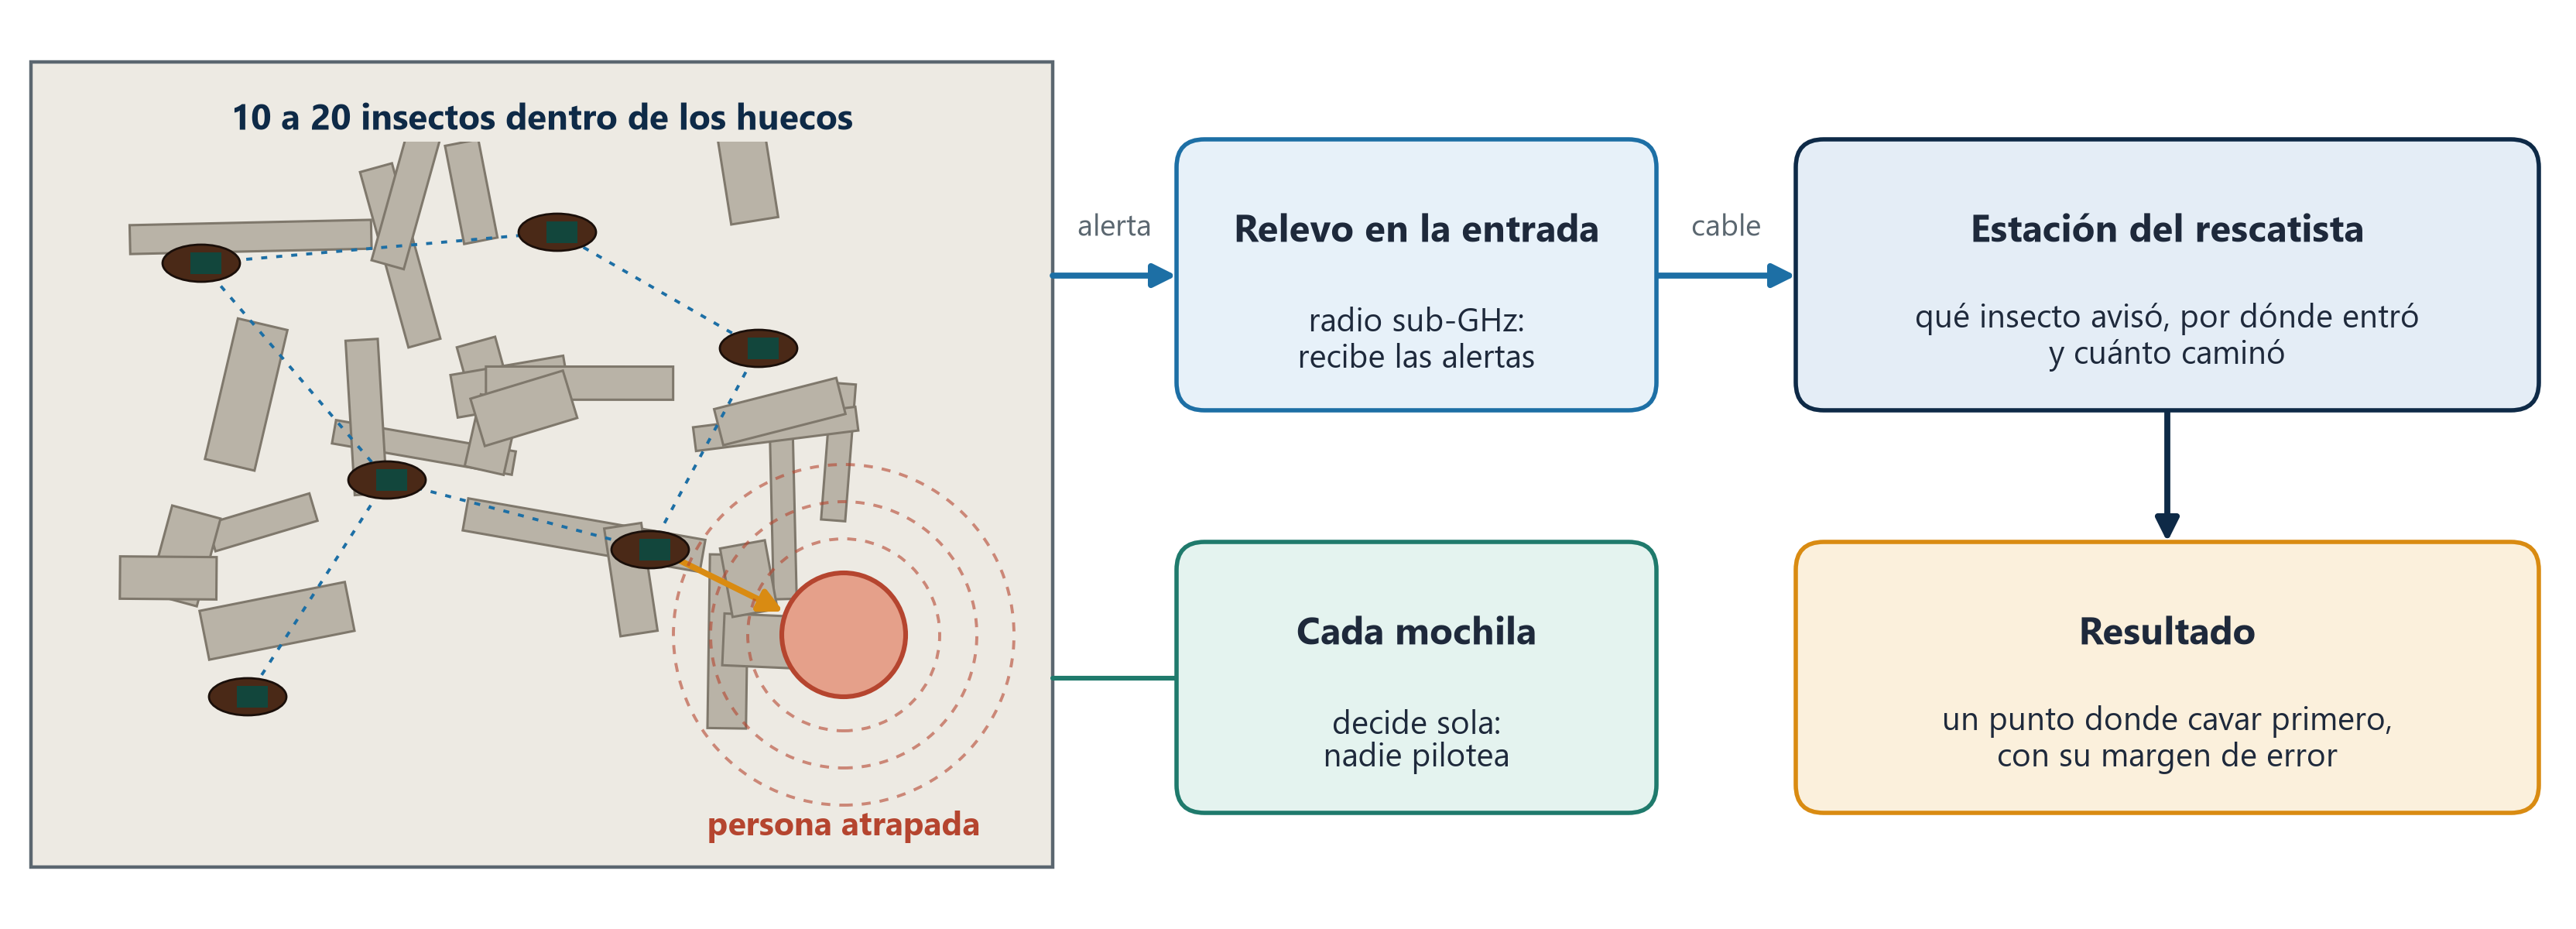
\includegraphics[width=0.96\textwidth]{figs/sistema.png}
\caption{Sistema completo: del enjambre al rescatista.}
\label{fig:sistema}
\end{figure}

\subsection{Caso 2: la red de tres FPGA}
\label{sec:casored}

El banco \sig{tb\_tri} recorre nueve escenarios (tabla~\ref{tab:escenarios}). En siete de ellos también lee los seis
displays de cada tarjeta, para revisar lo mismo que vería una persona.

\begin{table}[!htb]
\centering\footnotesize
\caption{Los nueve escenarios de la red. Resultado: 9 de 9 correctos.}
\label{tab:escenarios}
\rowcolors{2}{SoftGray}{white}
\begin{tabularx}{\textwidth}{@{}>{\bfseries}c >{\raggedright\arraybackslash}p{3.1cm} >{\raggedright\arraybackslash}X@{}}
\toprule
\rowcolor{TableHead} N.º & Escenario & Qué se comprueba y qué se midió \\
\midrule
1 & Triangulación con puente & A a 32.00~m, fuera de alcance, y B a 31.56~m. El aviso de A llega por B; conteo 2 en las tres; persona a 6.2~cm de la real, 1.10~s después del encendido. Displays: \sig{APd2b-}, \sig{bPd2Ar}, \sig{rPd2-b} \\
2 & Objeto caliente y bordes & 47~\textdegree C no cuenta. 34 y 39~\textdegree C no detectan; 35 y 38~\textdegree C sí \\
3 & Una sola mochila & A detecta; B, sin detectar, hace de puente. Conteo 1 en las tres \\
4 & Rumbos opuestos & Las rectas no se cruzan: el receptor lo indica y promedia \\
5 & Botón & Nada caliente; botón de B: conteo 1 en las tres, en la posición de la mochila \\
6 & Sin alcance & Las mochilas se oyen a 18~m, pero ninguna llega al receptor. Conteo 2, 2 y 0 \\
7 & Seguir al sensor & Al salir de la ventana el conteo baja y al volver sube: 2, 1, 0, 1 (figura~\ref{fig:seguimiento}) \\
8 & Ruido en la línea & Tres segundos de pulsos: 16 tramas descartadas por CRC y 18 perdidas contadas por secuencia; ningún dato equivocado \\
9 & Corte del alcance & A 31.00~m se oye por los dos ejes; a 32.00~m, no. En diagonal, a 31.96~m sí y a 32.0005~m no (figura~\ref{fig:umbral}) \\
\bottomrule
\end{tabularx}
\end{table}

\begin{figure}[!htb]
\centering
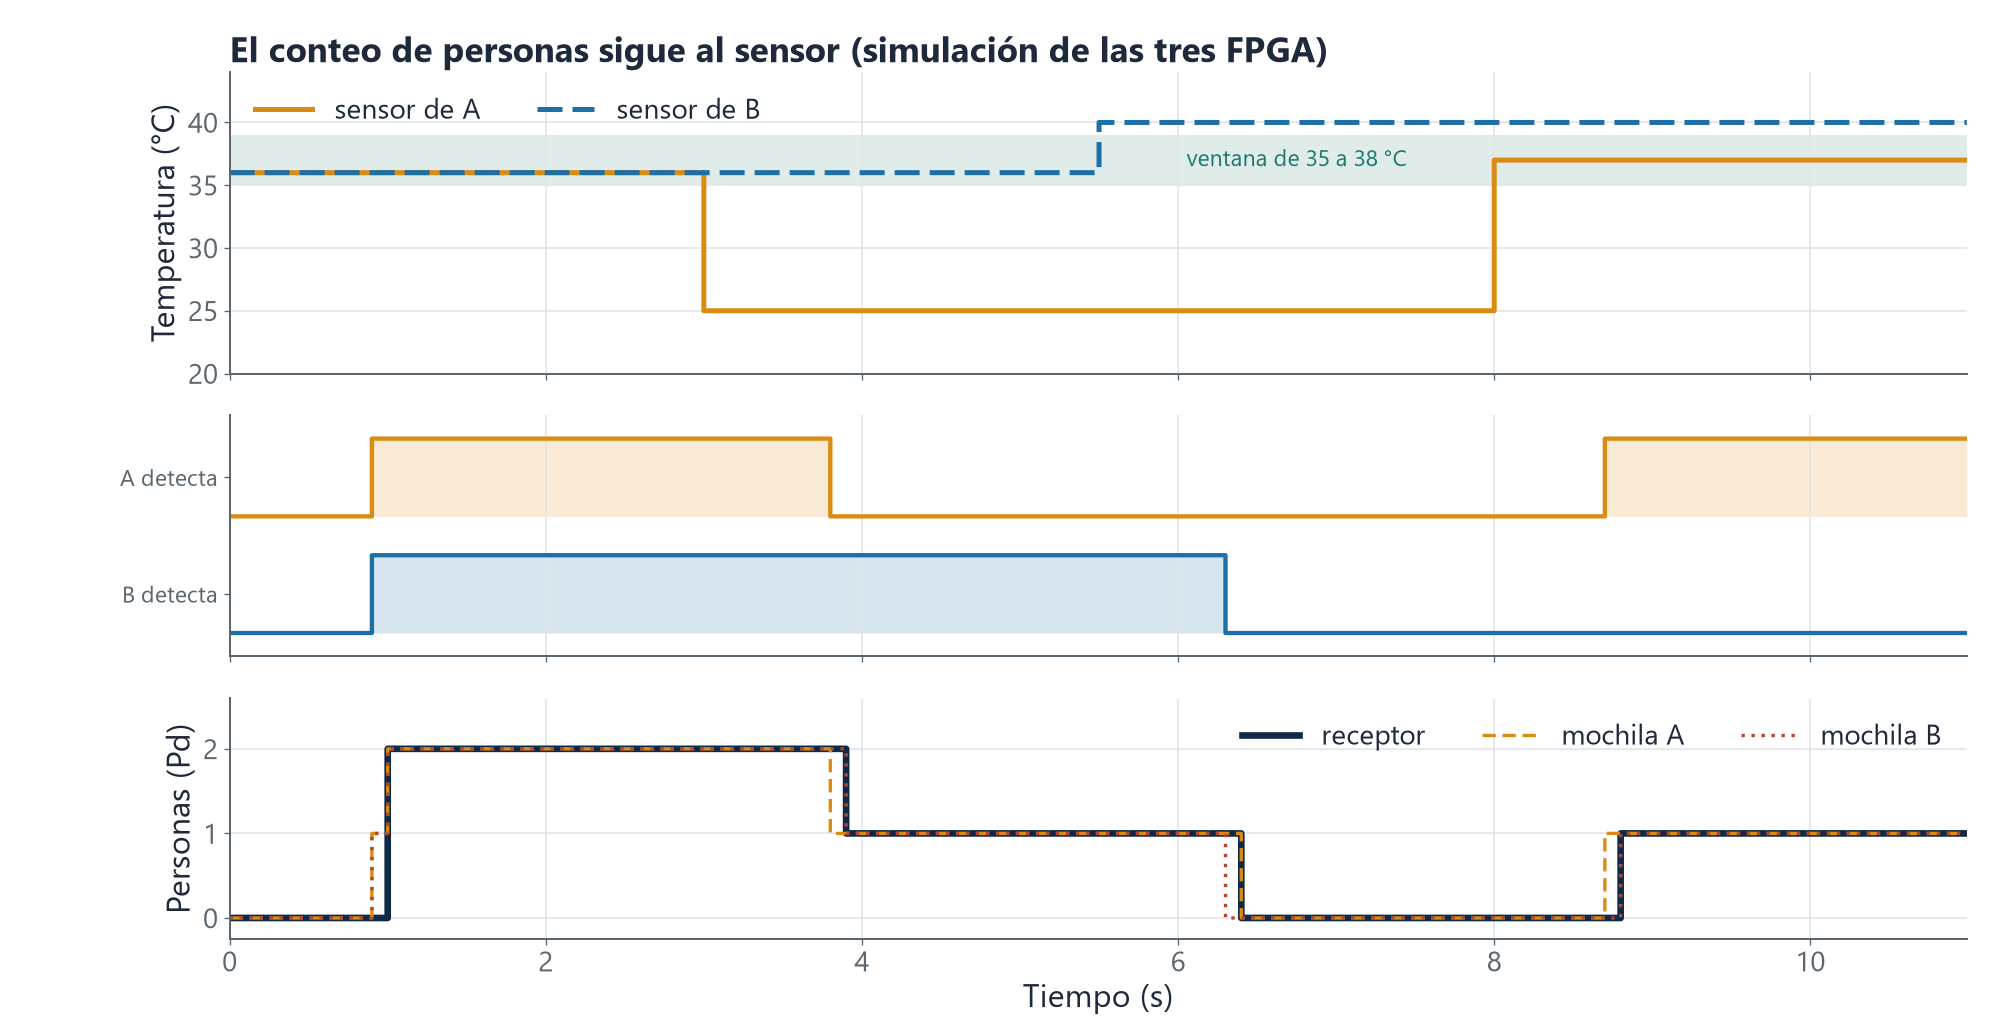
\includegraphics[width=0.88\textwidth]{figs/red_seguimiento.png}
\caption{Escenario 7, con datos de la simulación del circuito. La detección aparece y desaparece unos 0.8~s después
del cambio de temperatura.}
\label{fig:seguimiento}
\end{figure}

\begin{figure}[!htb]
\centering
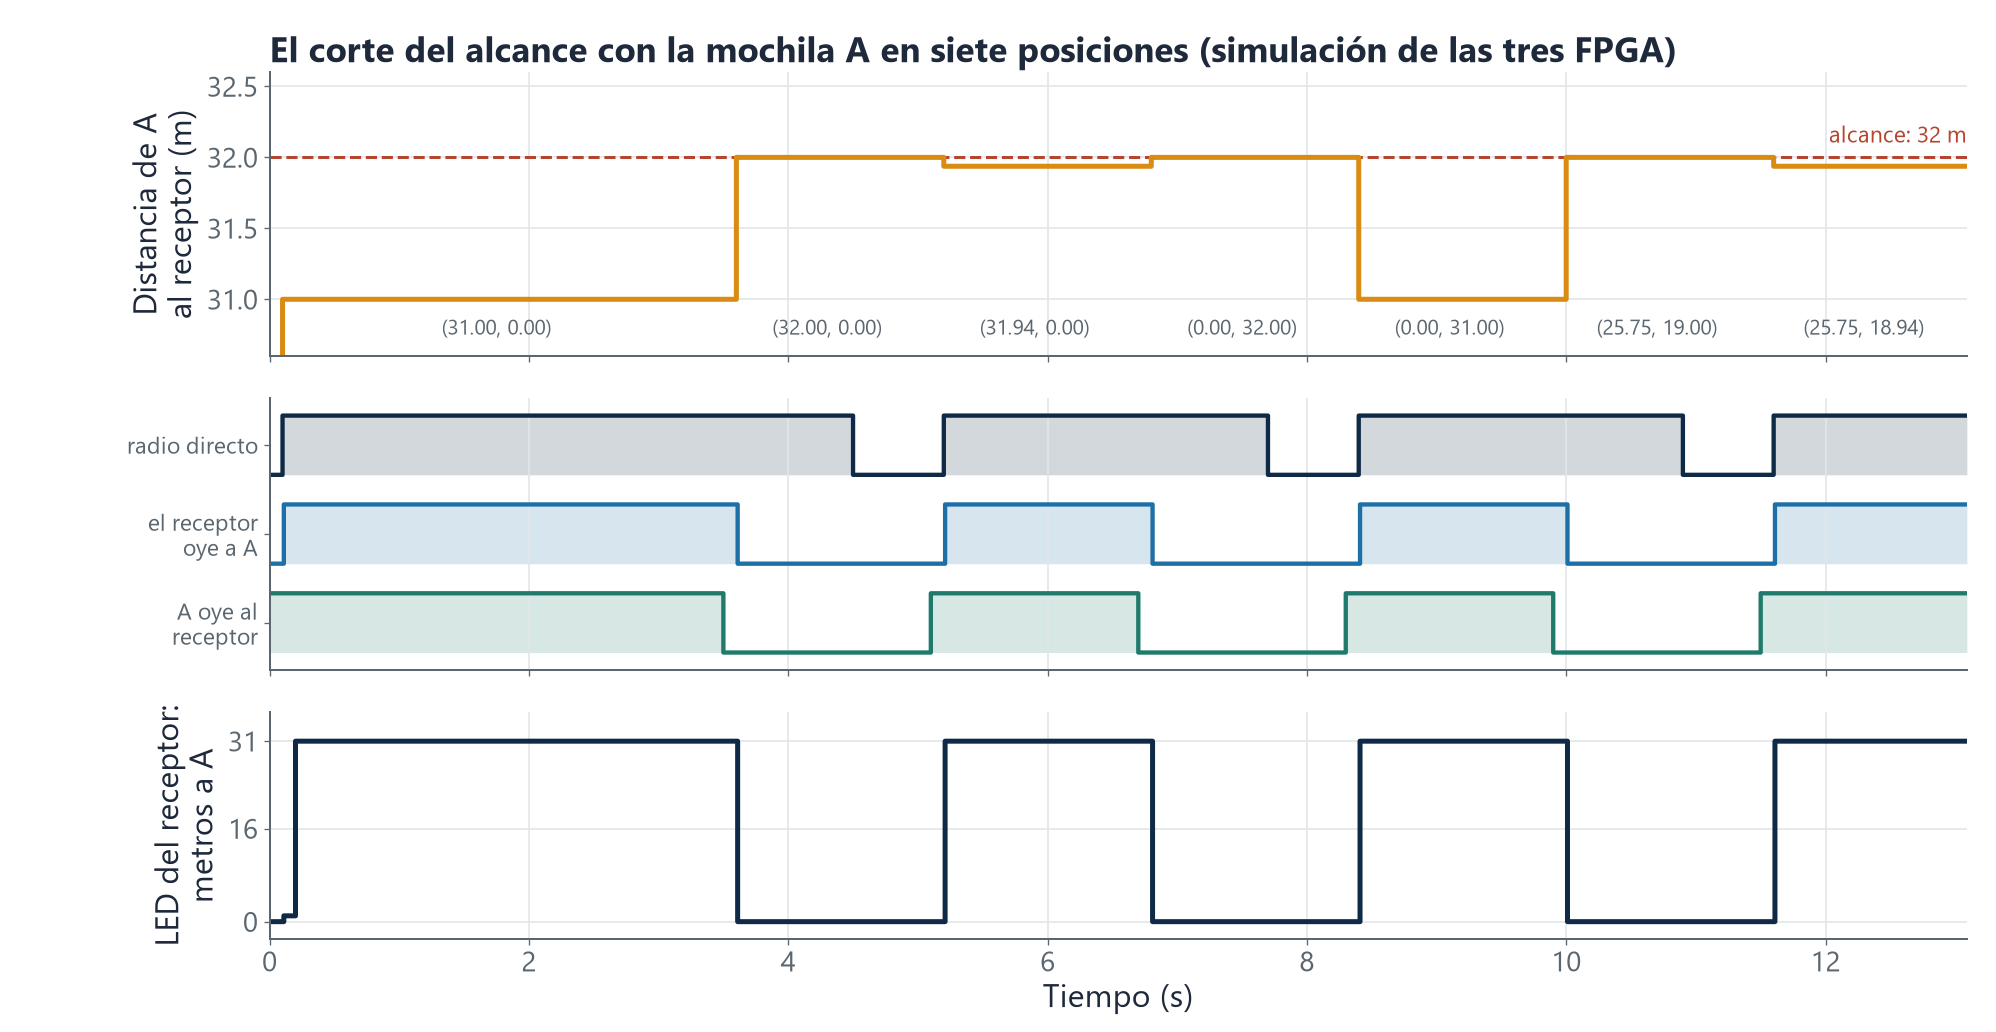
\includegraphics[width=0.88\textwidth]{figs/red_umbral.png}
\caption{Escenario 9. Los tonos se pierden en cuanto la mochila pasa de 32~m; el enlace se da por perdido un segundo
después, cuando caduca la última trama.}
\label{fig:umbral}
\end{figure}

\textbf{La terminal del operador} la probamos contra las tres tarjetas simuladas y pasó 71 de 71 comprobaciones. Con las dos
detecciones activas, el operador ve algo como esto:

\noindent\begin{minipage}{\textwidth}\scriptsize
\begin{verbatim}
PERSONAS DETECTADAS: 2     Persona estimada en (25.56, 19.25) m  ->  TRIANGULADA (dos rumbos)
Mochila A   [radio: por el puente B]   posicion (25.75, 19.00) m, a 32.00 m del receptor
            termica SI, 36 C | boton no | ALERTAR | pixeles calientes 14 | rumbo 133.6 grados
Mochila B   [radio: directo]   posicion (25.25, 19.00) m, a 31.56 m del receptor
            termica SI, 37 C | boton no | ALERTAR | pixeles calientes 12 | rumbo 43.2 grados
Receptor    tonos: oye a A (1 kHz) no [potencia 43], oye a B (2 kHz) SI [potencia 27600]
            distancia entre A y B 0.50 m | LED 00000 11111 (A: no se oye | B: 31 m)
Enlace      tramas perdidas: de A 0, de B 0 | descartadas por CRC 0
\end{verbatim}
\end{minipage}


\begin{table}[!htb]
\centering\footnotesize
\caption{Síntesis de la red en Quartus 24.1 (49\,760 elementos lógicos), reloj de 50~MHz. Peor caso: modelo lento,
85~\textdegree C.}
\label{tab:sintesisred}
\rowcolors{2}{SoftGray}{white}
\begin{tabularx}{\textwidth}{@{}>{\bfseries\raggedright\arraybackslash}X r r r r r@{}}
\toprule
\rowcolor{TableHead} Variante & Elem. lógicos & Registros & Mult. 9 bits & $f_{\max}$ (MHz) & Holgura (ns) \\
\midrule
Mochila A & 3\,933 (8~\%) & 2\,279 & 43 & 55.43 & 1.96 \\
Mochila B & 3\,952 (8~\%) & 2\,279 & 43 & 58.52 & 2.91 \\
Receptor & 4\,929 (10~\%) & 2\,523 & 76 & 61.63 & 3.77 \\
Receptor con la mochila B & 7\,525 (15~\%) & 4\,060 & 107 & 59.42 & 3.17 \\
\bottomrule
\end{tabularx}
\end{table}

\textbf{En las tarjetas.} El 18 de noviembre de 2026 corrimos seis escenarios correctos en las tres DE10-Lite con la versión
anterior del enlace (mapa de 20~m, suma de verificación y sin tonos). Obtuvimos 2.8~cm de error y el aviso de A llegó por el
puente; el sensor simulado detectó con 35, 36 y 38~\textdegree C y no con 34, 39, 47 ni 22~\textdegree C. El 23 de noviembre
cargamos la versión que aquí se describe y repetimos en las tarjetas los escenarios 1 a 7 y el 9, con entradas fijadas por
JTAG. Todas las comprobaciones salieron como en la simulación, y la triangulación dio 6.3~cm de error. No fue en una sola
corrida: a media prueba se perdió la conexión USB del receptor, y tuvimos que recargarlo y seguir desde el escenario 4. El
escenario 8, el del ruido, solo está verificado en simulación.

\subsection{Caso 3: la misión simulada}
\label{sec:resultados}

Cada misión libera a los insectos por un boquete de un colapso sintético con unos \areaLibre~m$^2$ de huecos; la
persona está inmóvil, a un recorrido medio de \distVictima~m. Cada configuración se corrió \numCorridas{} veces en
\numMapas{} colapsos: \numMisiones{} misiones de una hora, con un margen de unos $\pm5$ puntos (95~\%).

\textbf{Validación.} En una arena de $1\times1$~m el insecto simulado camina \valAndaNat{} del tiempo sin estímulos
(publicado: $0.37\pm0.20$), hace pausas de \valPausaNat~s ($36.8\pm24.1$) y suelta la pared con probabilidad
\valSalidaNat{} (0.005); con comandos, \valAndaCom{} (0.643) y \valSalidaCom{}
(0.052)~\cite{dirafzoon2017,tranngoc2024}. Solo difiere la pausa con comandos: \valPausaCom~s frente a 5.6~s, de modo
que el modelo es conservador (tabla~\ref{tab:validacion}).

\begin{table}[!htb]
\centering\footnotesize
\caption{Marcha simulada frente a la publicada.}
\label{tab:validacion}
\rowcolors{2}{SoftGray}{white}
\begin{tabularx}{0.86\textwidth}{@{}>{\raggedright\arraybackslash}X r r@{}}
\toprule
\rowcolor{TableHead} \textbf{Medida} & \textbf{Publicado} & \textbf{Simulación} \\
\midrule
Fracción del tiempo caminando, sin estímulos & $0.37\pm0.20$ & \valAndaNat \\
Pausa media, sin estímulos (s) & $36.8\pm24.1$ & \valPausaNat \\
Probabilidad de soltar la pared, sin estímulos & 0.005 & \valSalidaNat \\
Fracción del tiempo caminando, con comandos & 0.643 & \valAndaCom \\
Probabilidad de soltar la pared, con comandos & 0.052 & \valSalidaCom \\
Pausa media, con comandos (s) & 5.55 & \valPausaCom \\
\bottomrule
\end{tabularx}
\end{table}

\textbf{Cuatro políticas.} La \textbf{pasiva} solo detecta; la \textbf{antipausa} da un pulso de avance cuando el
insecto lleva 15~s quieto; la \textbf{estocástica} añade giros al azar, y la \textbf{guiada}, la del núcleo, gira
además hacia el calor (figura~\ref{fig:politicas} y tabla~\ref{tab:politicas}); la figura~\ref{fig:mapa} muestra una
misión.

\begin{figure}[!htb]
\centering
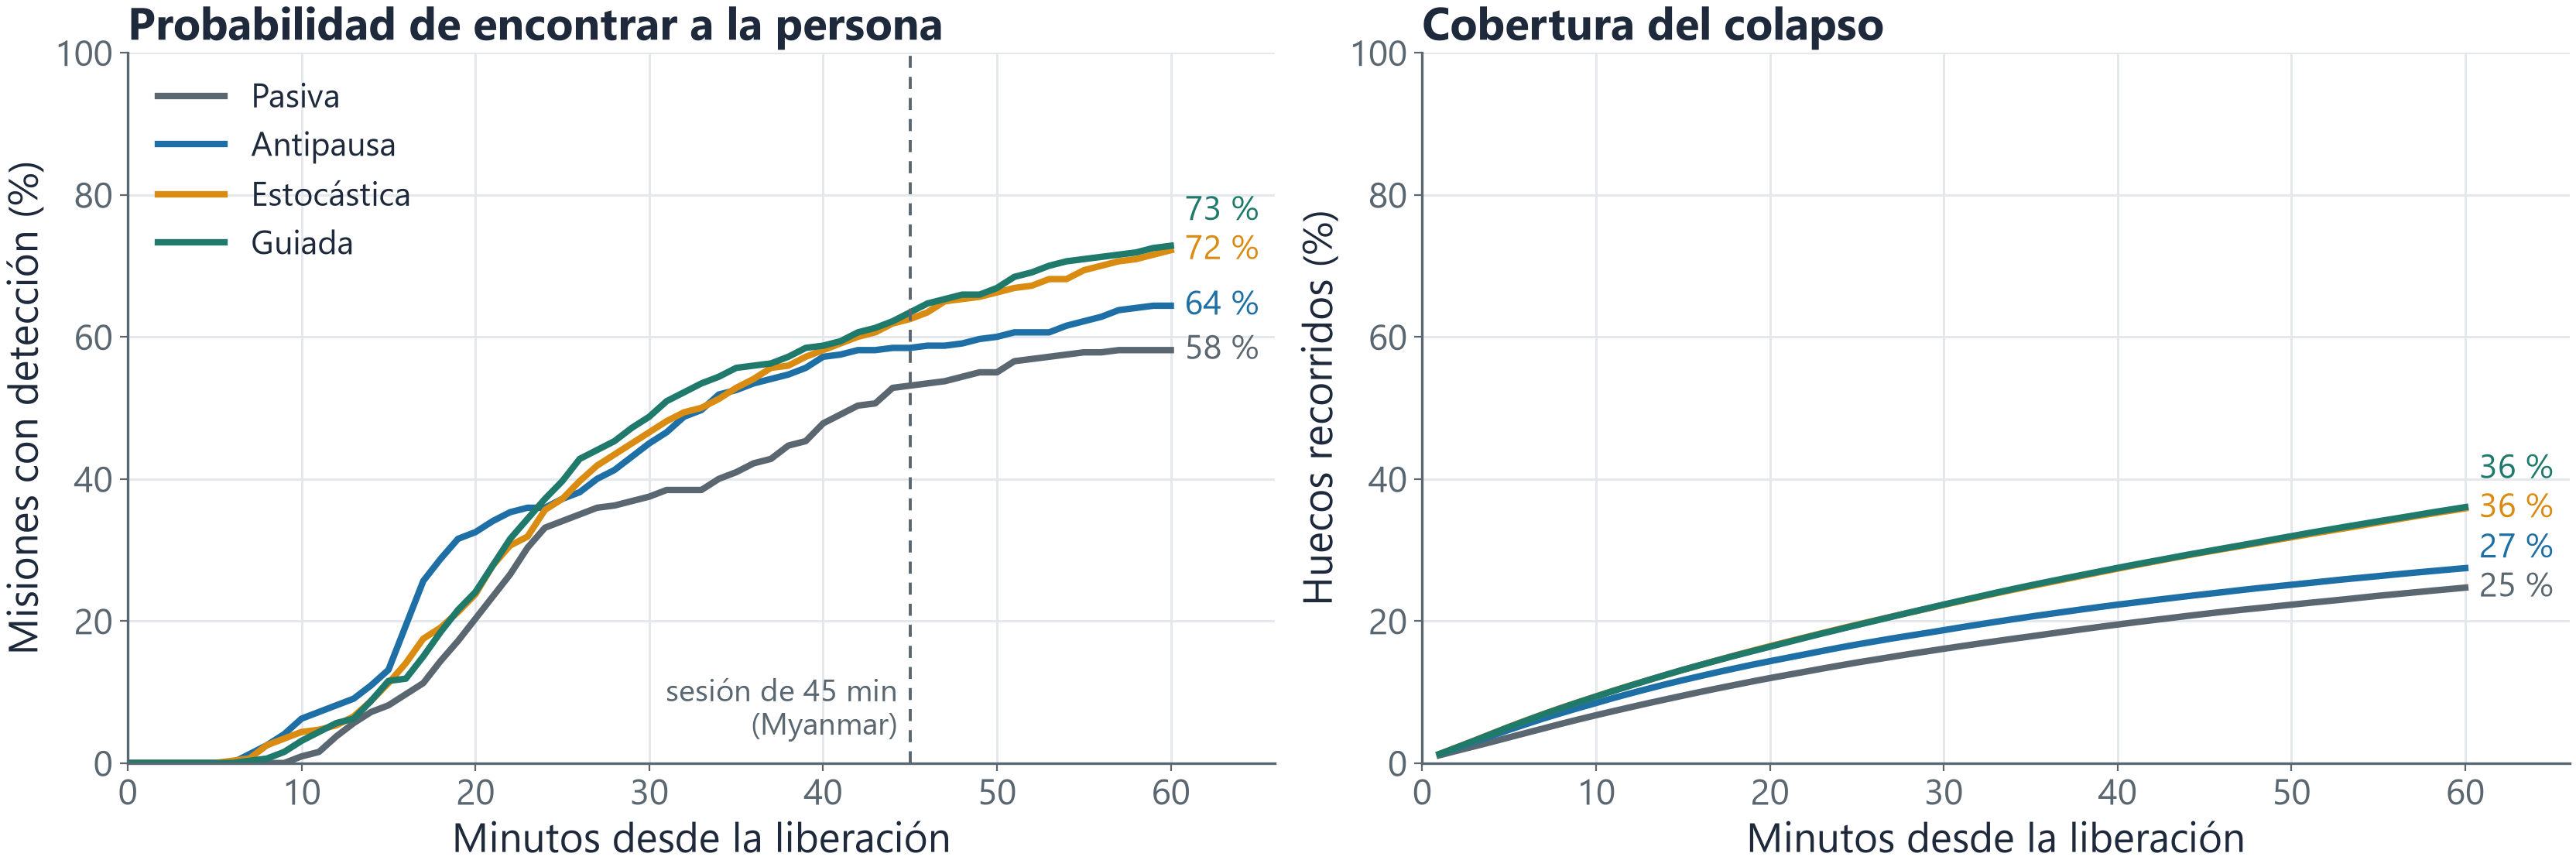
\includegraphics[width=0.98\textwidth]{figs/resultados_politicas.png}
\caption{Diez insectos, \numMisiones{} misiones por política. Izquierda: misiones en que algún insecto confirma a la
persona. Derecha: fracción de los huecos por los que pasó al menos un insecto.}
\label{fig:politicas}
\end{figure}

\begin{table}[!htb]
\centering\footnotesize
\caption{Resultados por política con diez insectos.}
\label{tab:politicas}
\rowcolors{2}{SoftGray}{white}
\begin{tabularx}{\textwidth}{@{}>{\bfseries\raggedright\arraybackslash}X r r r r r r r r@{}}
\toprule
\rowcolor{TableHead} & \multicolumn{4}{c}{\textbf{Detección acumulada (\%)}} & \textbf{Mediana} & \textbf{Cobertura} & \textbf{Estímulos por} & \textbf{Tiempo} \\
\rowcolor{TableHead} \textbf{Política} & 15 min & 30 min & 45 min & 60 min & (min) & (\%) & insecto y hora & caminando (\%) \\
\midrule
\tablaPoliticas
\bottomrule
\end{tabularx}
\end{table}

La ganancia viene de mantener al insecto en movimiento y despegarlo de las paredes; girar hacia el calor casi no
añade, porque solo actúa dentro del alcance de la matriz. En el primer cuarto de hora las políticas no se
distinguen, y el costo es bajo: unos \estGuiada{} estímulos por insecto y por hora.

\begin{figure}[!htb]
\centering
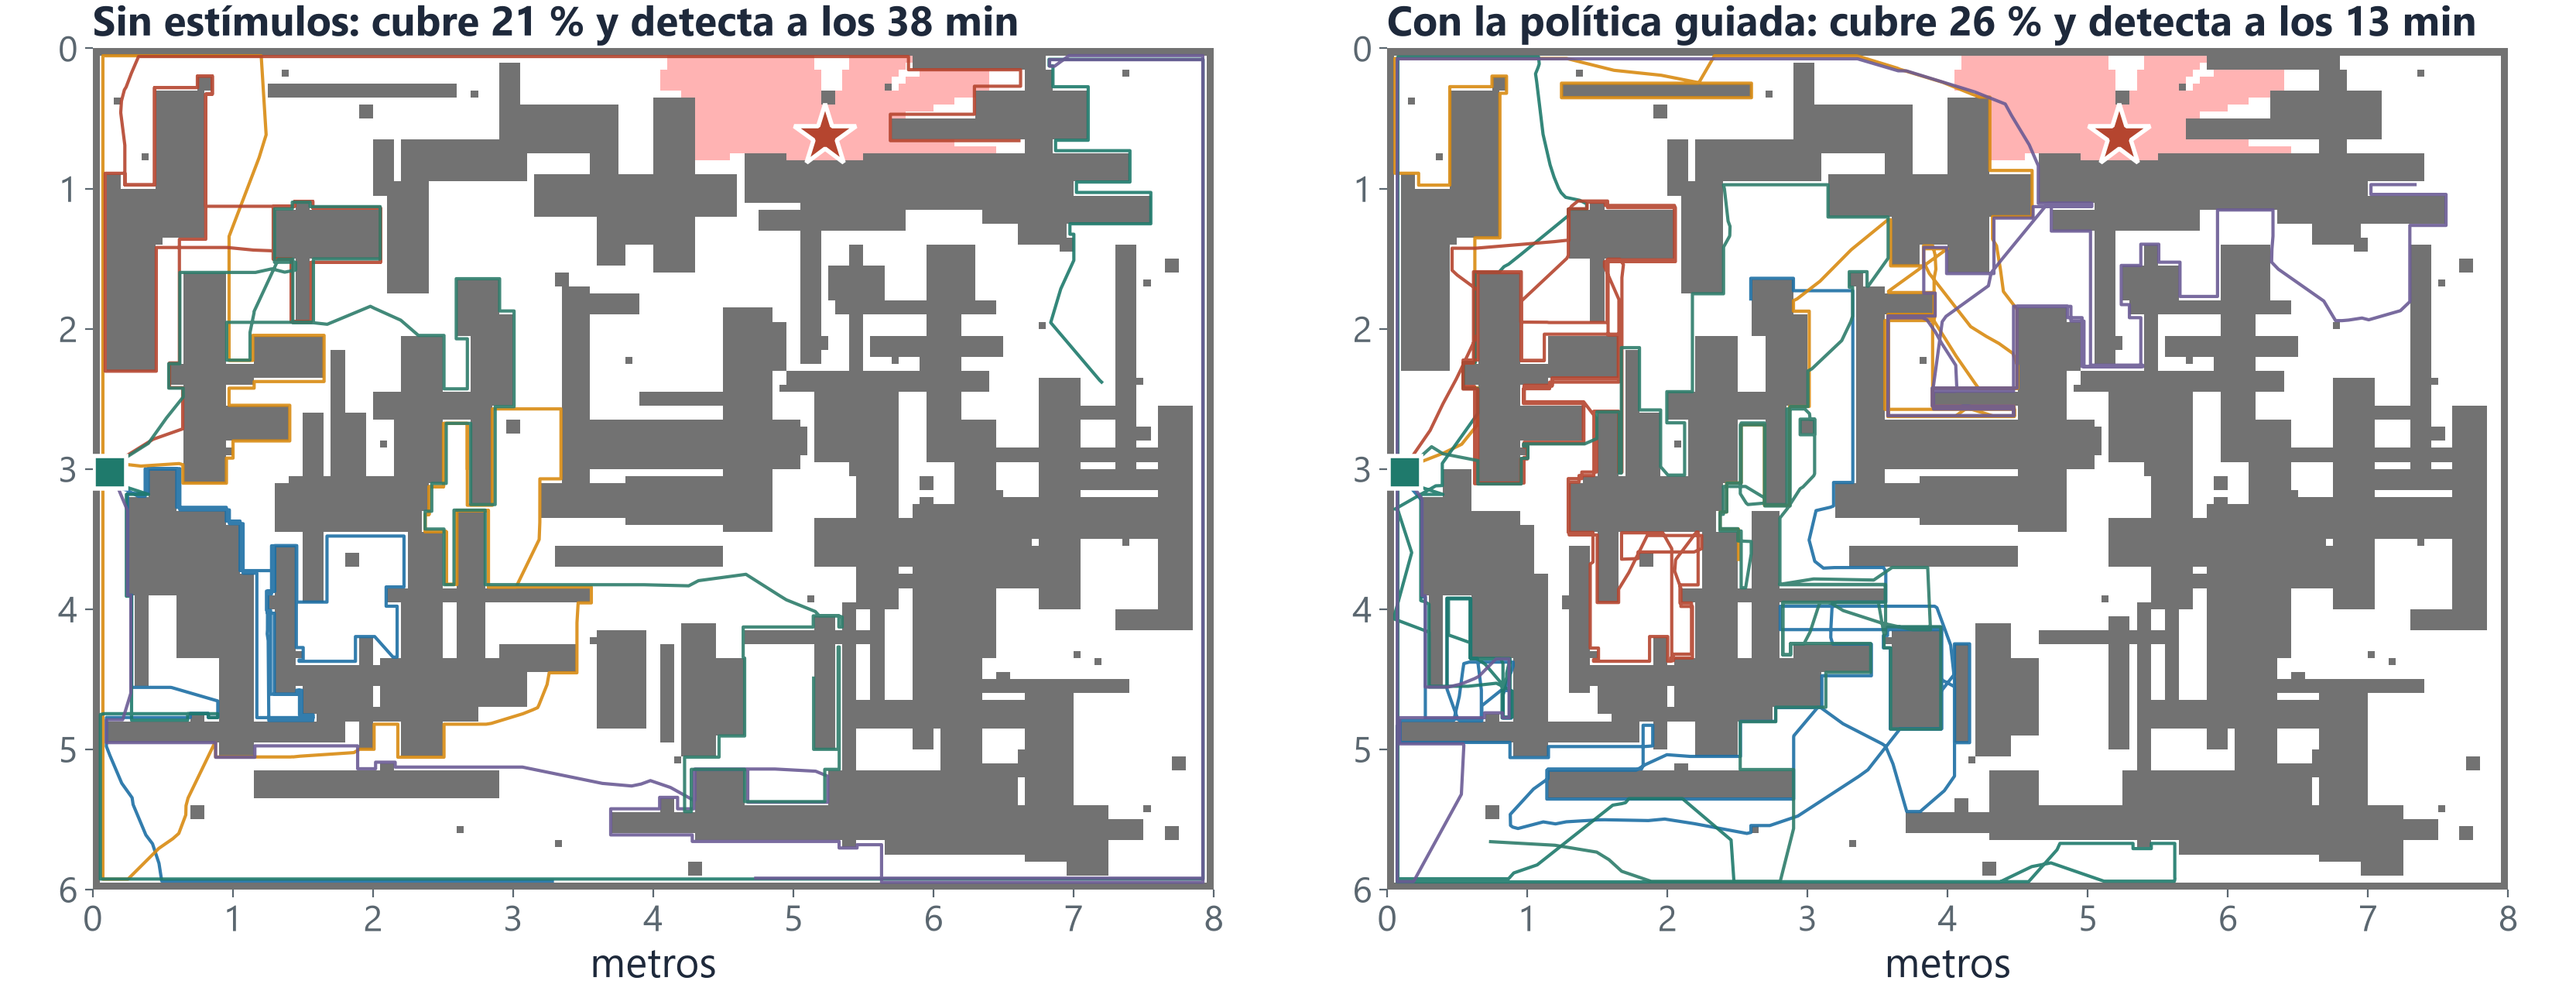
\includegraphics[width=0.92\textwidth]{figs/mapa_trayectorias.png}
\caption{Una misión de ejemplo: seis insectos durante 45~min en el mismo colapso. Cuadro verde: entrada; estrella:
persona; zona sombreada: desde donde la matriz confirma.}
\label{fig:mapa}
\end{figure}

\textbf{El colapso pesa más que la política} (figura~\ref{fig:mapaenjambre}a). Según el colapso, la detección en una
hora va de \mapaMinPasiva{} a \mapaMaxPasiva~\% sin estímulos y de \mapaMinGuiada{} a \mapaMaxGuiada~\% con la
guiada, que gana en \mapasGanaGuiada{} de los \numMapas{}, empata en \mapasEmpate{} y pierde en
\mapasPierdeGuiada. En el mejor caso pasa de \mapaMejorPasiva{} a \mapaMejorGuiada~\%; en el peor, de
\mapaPeorPasiva{} a \mapaPeorGuiada~\%, porque ahí seguir la pared lleva directo a la persona. Un enjambre mixto, con
cinco de cada uno, conserva el promedio (\mixtoSesenta~\%) y quita el caso malo (\mixtoPeor~\% en lugar de
\mapaPeorGuiada~\%): es la configuración que se recomienda.

\textbf{Tamaño del enjambre} (figura~\ref{fig:mapaenjambre}b). Uno solo encuentra a la persona en una de cada cuatro
misiones (\enjHoraPasivaUno{} y \enjHoraGuiadaUno~\%). Con veinte, la guía sube la detección de
\enjHoraPasivaVeinte{} a \enjHoraGuiadaVeinte~\%. Diez guiados (\enjHoraGuiadaDiez~\%) rinden como entre veinte y
cuarenta sin guiar: la política equivale a duplicar o triplicar el enjambre.

\begin{figure}[!htb]
\centering
\begin{subfigure}{0.50\textwidth}
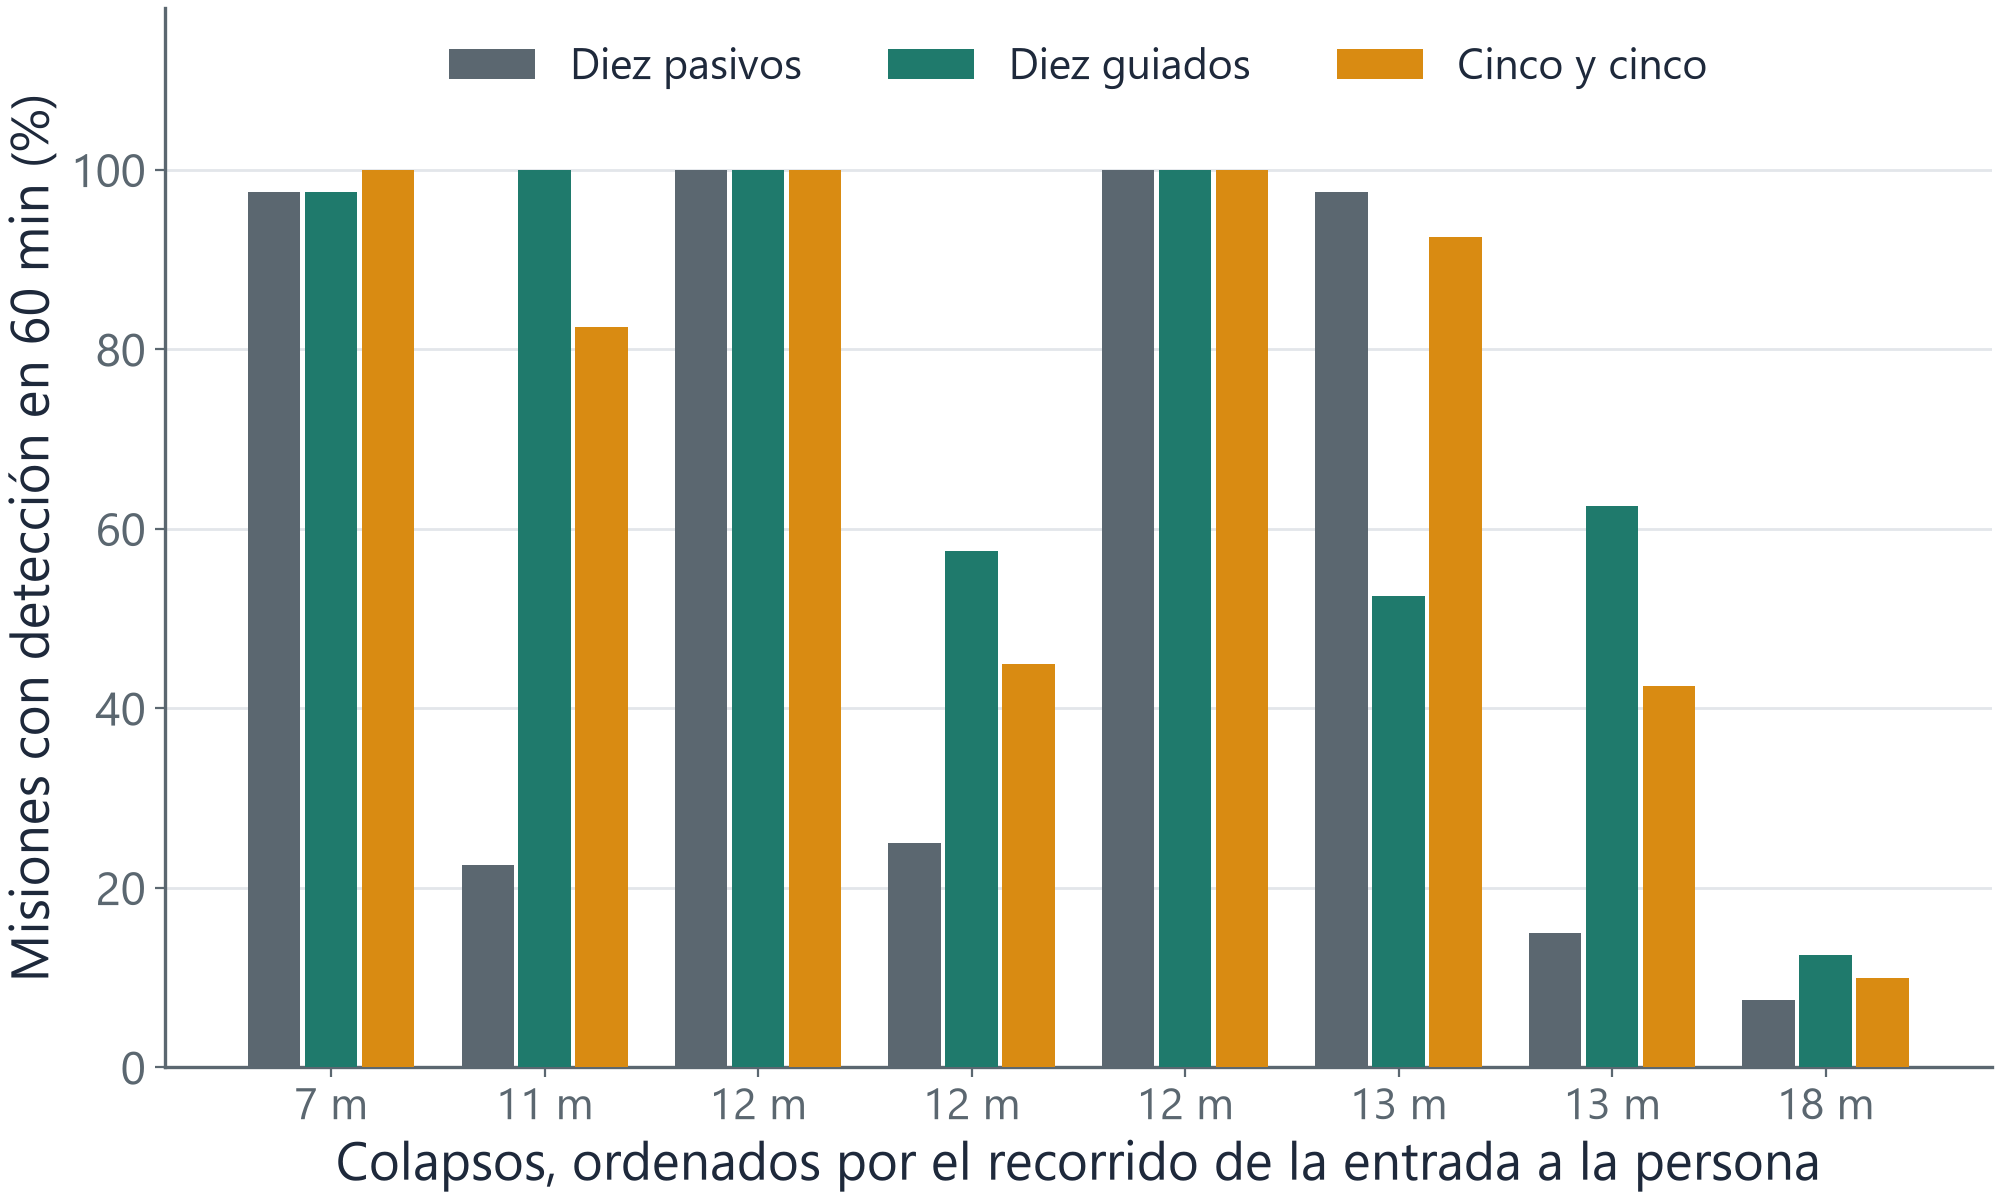
\includegraphics[width=\linewidth]{figs/por_mapa.png}
\caption{Detección a 60~min en cada colapso.}
\end{subfigure}\hfill
\begin{subfigure}{0.46\textwidth}
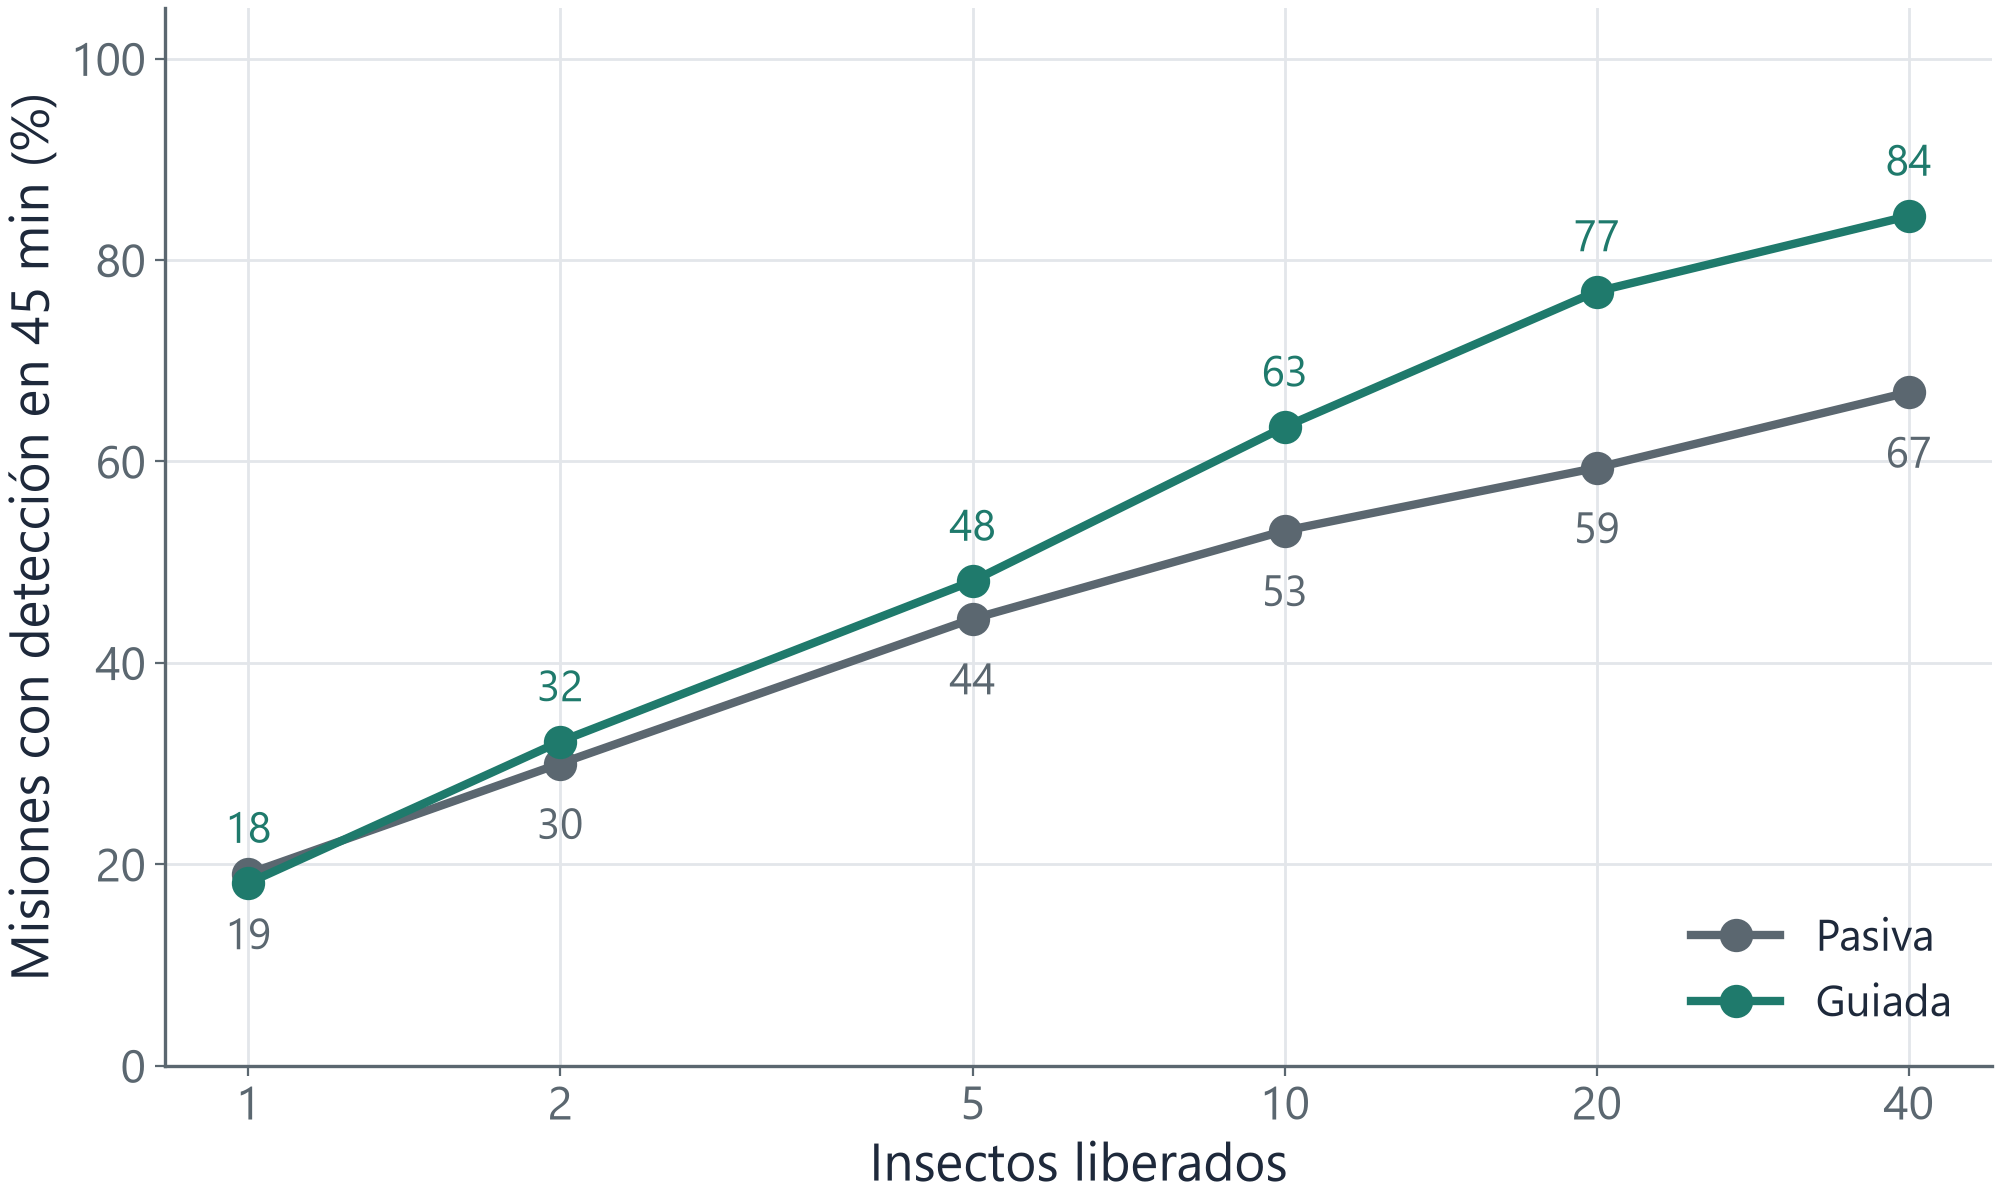
\includegraphics[width=\linewidth]{figs/enjambre.png}
\caption{Detección a 45~min según el número de insectos.}
\end{subfigure}
\caption{Efecto de la geometría del colapso y del tamaño del enjambre.}
\label{fig:mapaenjambre}
\end{figure}

\textbf{Sensor y habituación.} Con la guiada, la matriz de $8\times8$ detecta en una hora en \senOchoSesenta~\% de las
misiones y la de $32\times32$ en \senTreintaDosSesenta~\%: la que se consigue en México pierde pocos puntos. En
misiones de dos horas con pulsos unipolares, estimular sin límite aplica \habEstSinLimite{} estímulos por insecto y
por hora y deja la respuesta en \habRespSinLimite~\%; con el presupuesto son \habEstDosificado{} y
\habRespDosificado~\%, con una detección prácticamente igual (\habDetSinLimite{} y \habDetDosificado~\%). El
argumento para dosificar es el animal, no el rendimiento (figura~\ref{fig:sensorhab}).

\begin{figure}[!htb]
\centering
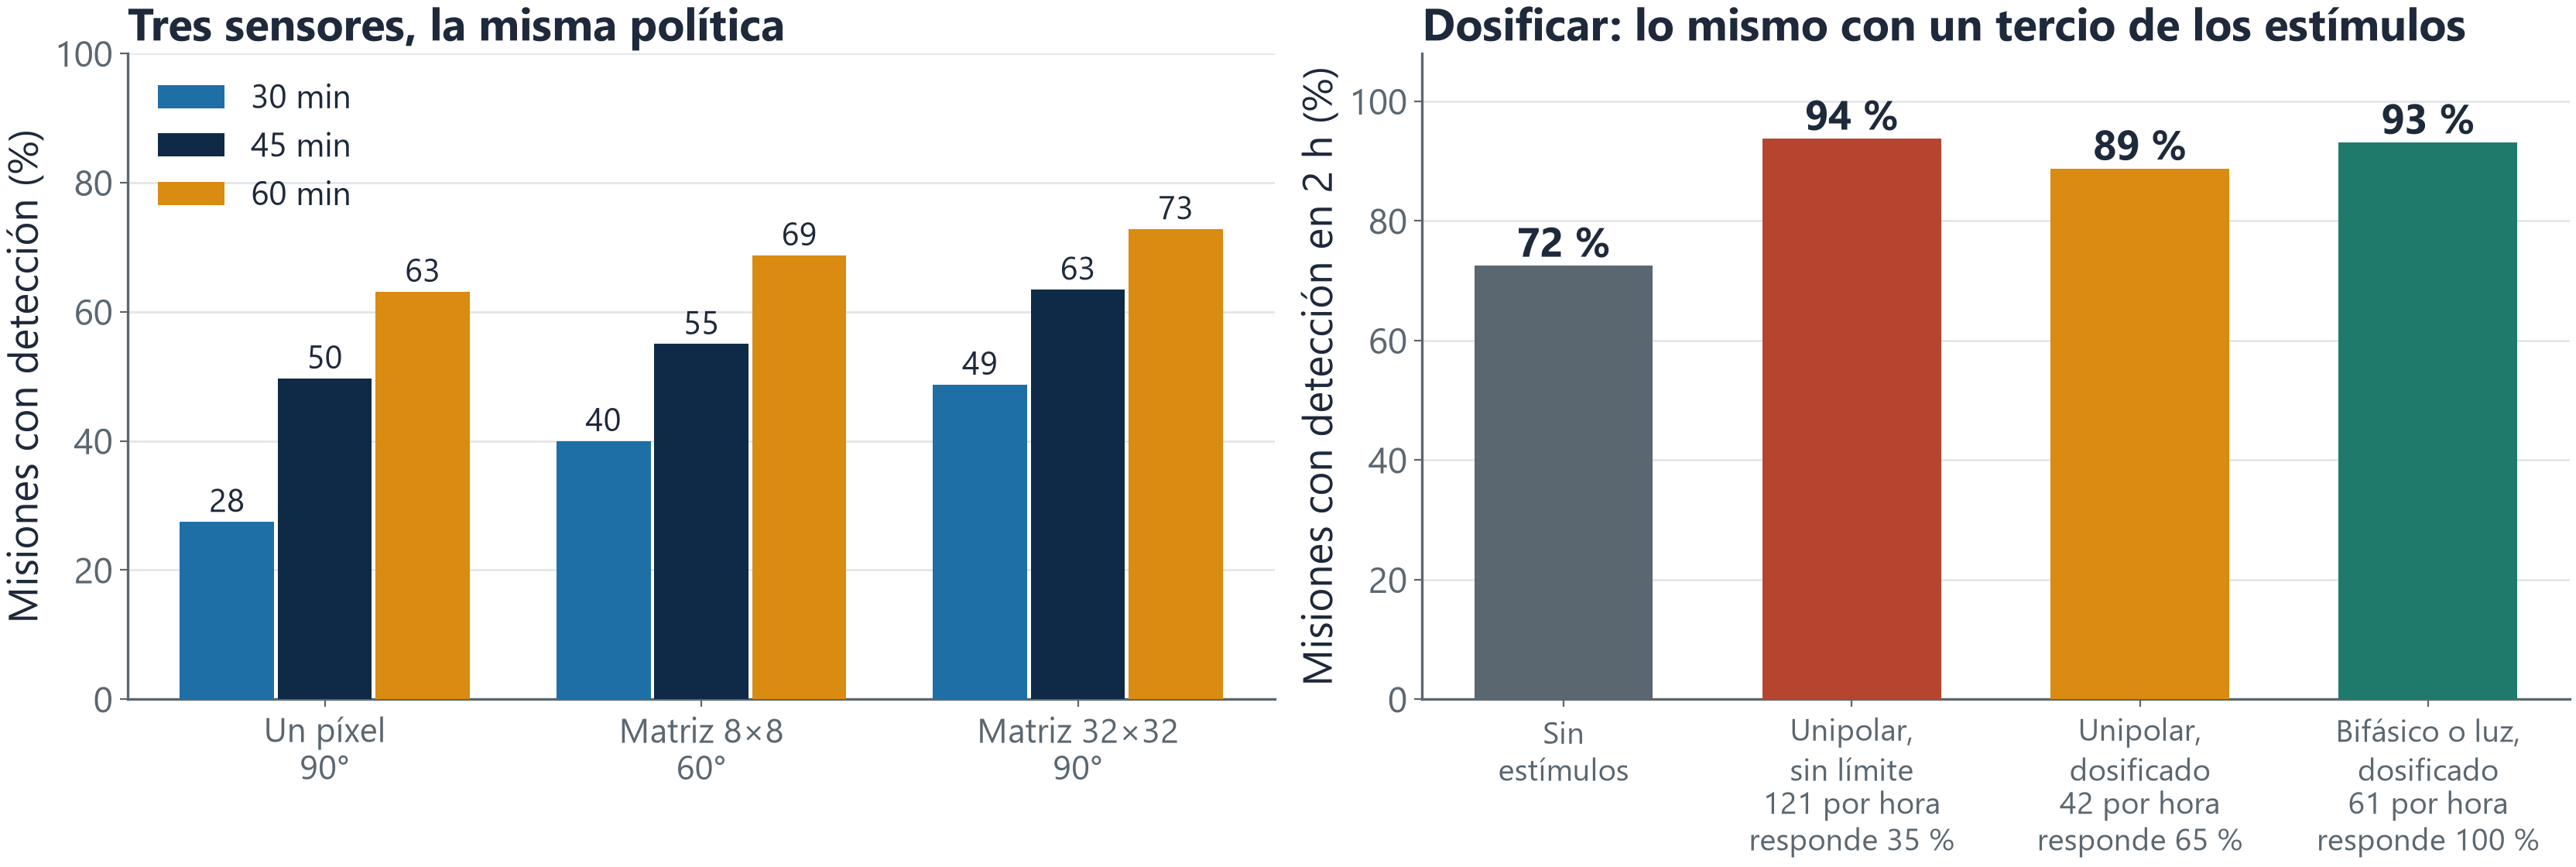
\includegraphics[width=0.94\textwidth]{figs/sensores_habituacion.png}
\caption{Izquierda: política guiada con tres sensores. Derecha: misiones de dos horas con pulsos unipolares, con y
sin dosificación, frente a un estímulo que no habitúa.}
\label{fig:sensorhab}
\end{figure}

\textbf{Sensibilidad} (figura~\ref{fig:sensibilidad}). Doce supuestos se movieron uno a la vez en cuatro colapsos.
Cuatro cambian el resultado más que el margen de muestreo: el largo del tramo recto (de \sensTramoBajoGuiada{} a
\sensTramoAltoGuiada~\%), la velocidad que quita la carga (de \sensCargaBajoGuiada{} a \sensCargaAltoGuiada~\% si
resta 30~\%), la duración de las pausas (de \sensPausaBajoGuiada{} a \sensPausaAltoGuiada~\%) y la velocidad de
marcha (de \sensVelocidadBajoGuiada{} a \sensVelocidadAltoGuiada~\%). La política tolera la incertidumbre sobre el
estímulo, que es lo peor conocido; lo que más importa es cuánto y qué tan rápido camina el insecto.

\begin{figure}[!htb]
\centering
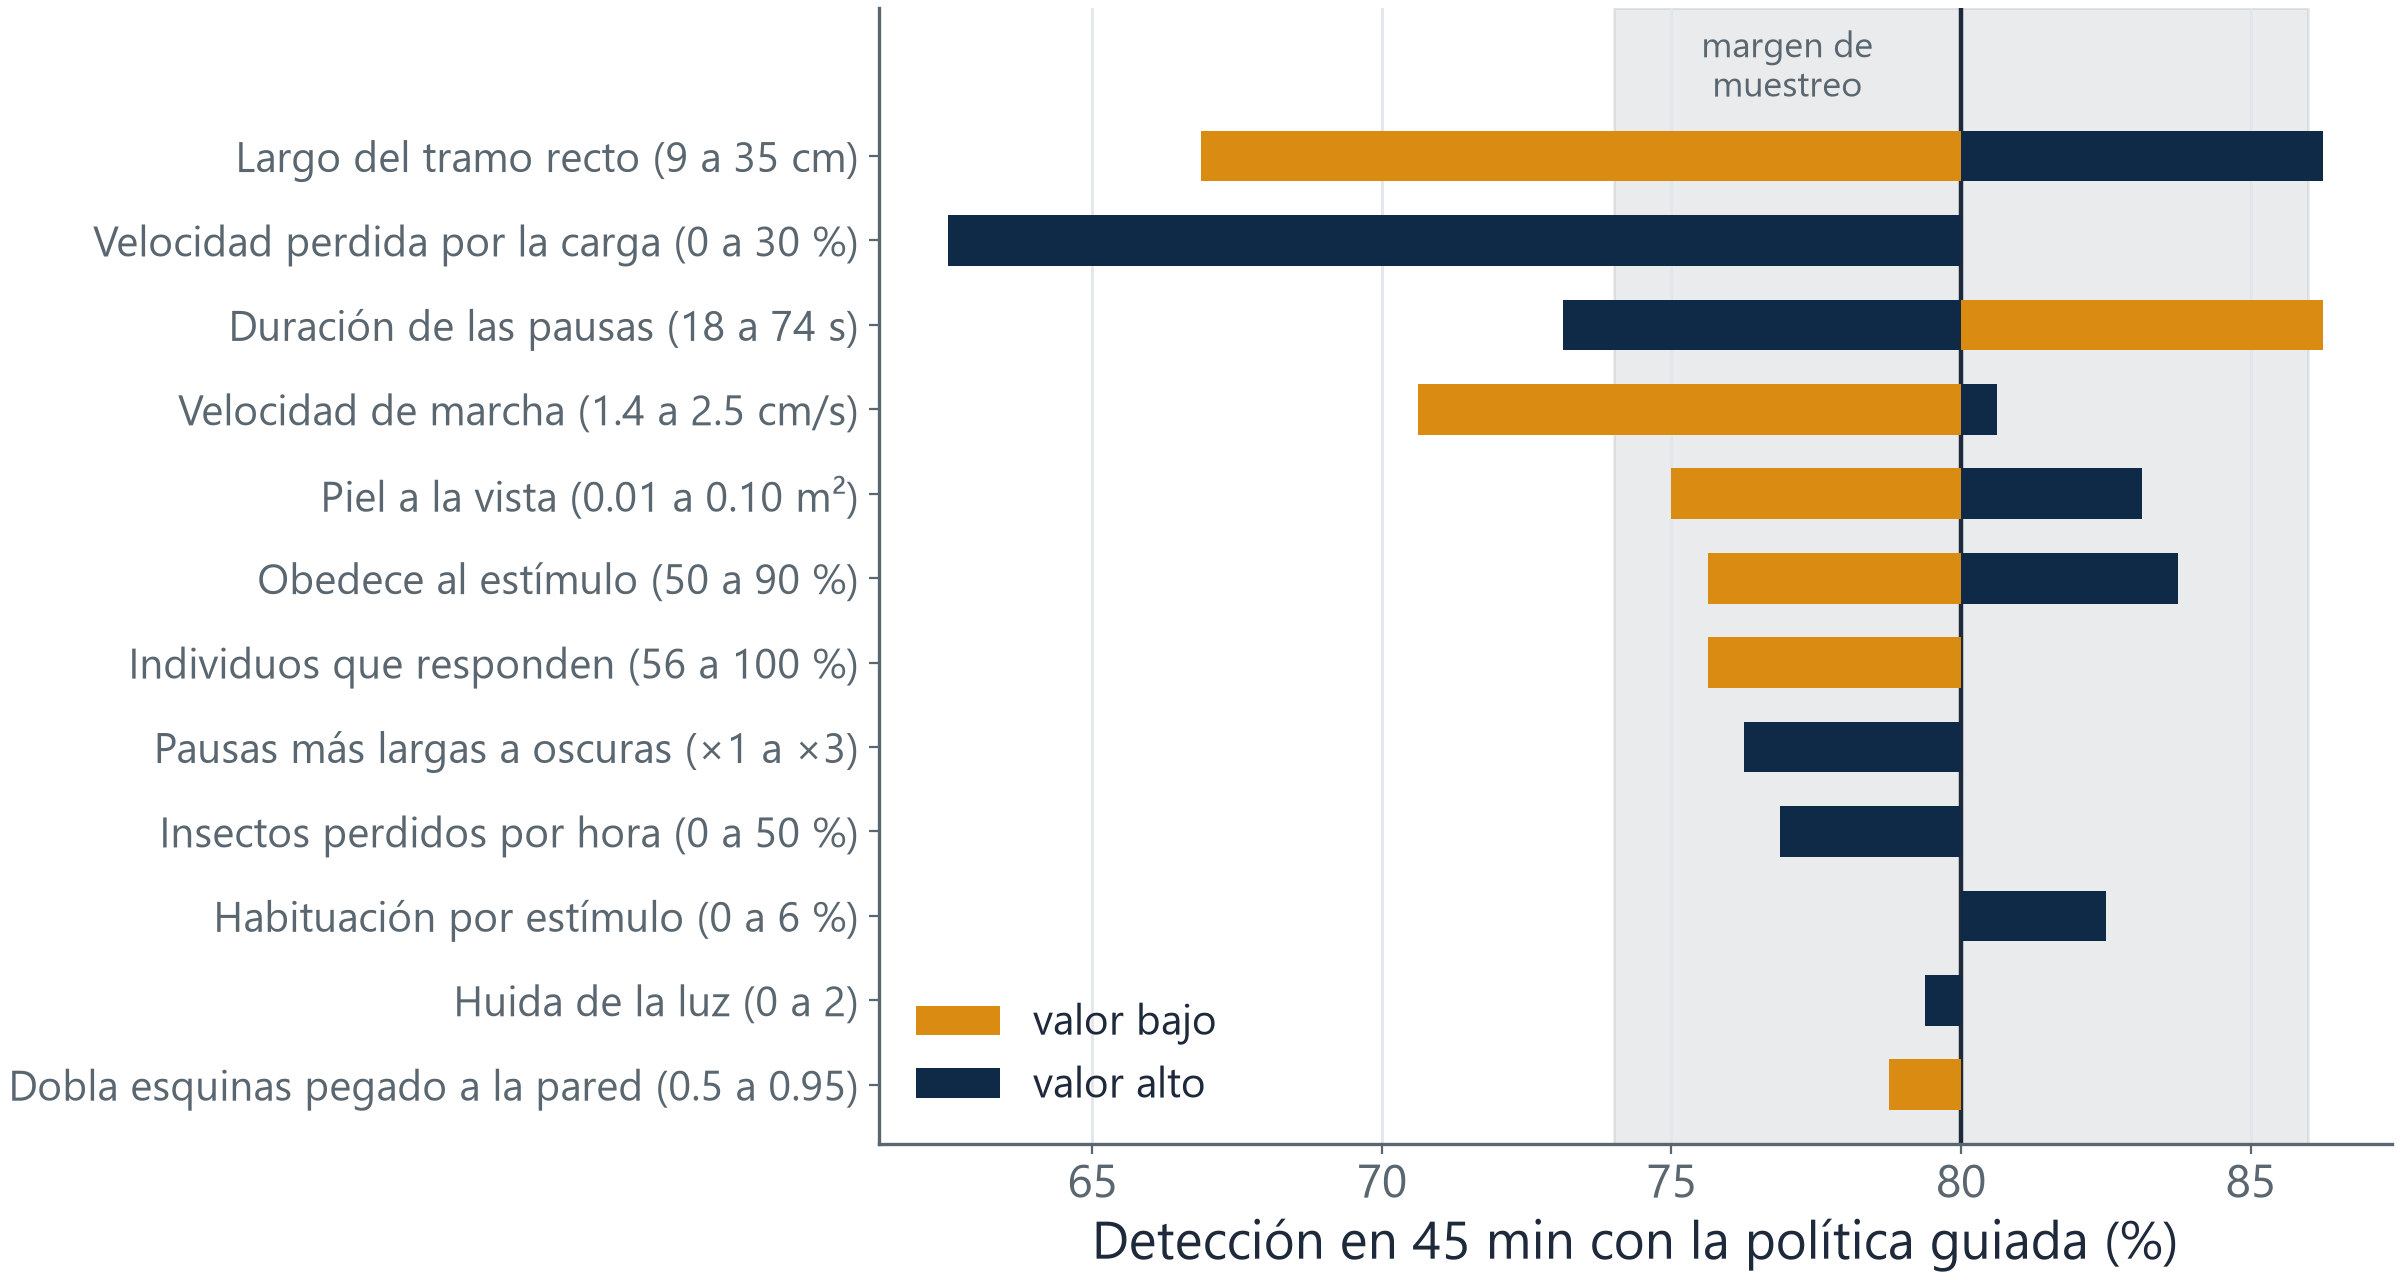
\includegraphics[width=0.78\textwidth]{figs/sensibilidad.png}
\caption{Cambio en la detección a 45~min de la política guiada al mover cada supuesto.}
\label{fig:sensibilidad}
\end{figure}

\textbf{Recuperar a los insectos.}\phantomsection\label{sec:regreso} Tras 45~min de búsqueda se da la orden de
regreso; en el boquete hay un refugio oscuro que retiene a los que pasan a 30~cm (figura~\ref{fig:regreso}
y tabla~\ref{tab:regreso}, \regInsectos{} insectos por caso). Con solo el refugio vuelve \regTrampaSesenta~\% en una hora y \regTrampaDos~\% en
dos. Guiarlo a ciegas es peor: el rumbo recto o desandar la ruta recuperan \regRumboDos{} y \regRutaDos~\%, porque la
cuenta de pasos y giros se desvía con cada metro. Lo que cambia el resultado es una señal en la entrada: con un faro
infrarrojo que se percibe hasta 6~m y dos fotodiodos vuelve \regFaroSesenta~\% en una hora y \regFaroDos~\% en dos,
con \regEstFaro{} estímulos. Ningún método los recupera a todos. El faro es un supuesto: existen sus dos piezas por
separado, una cerca invisible~\cite{latif2014} y la localización de sonido desde la mochila~\cite{latif2016}.

\begin{table}[!htb]
\centering\footnotesize
\caption{Insectos recogidos (\%) después de la orden de regreso y estímulos gastados en volver.}
\label{tab:regreso}
\rowcolors{2}{SoftGray}{white}
\begin{tabularx}{0.9\textwidth}{@{}>{\raggedright\arraybackslash}X r r r r@{}}
\toprule
\rowcolor{TableHead} \textbf{Forma de regresar} & \textbf{30 min} & \textbf{60 min} & \textbf{120 min} & \textbf{Estímulos por insecto} \\
\midrule
\tablaRegreso
\bottomrule
\end{tabularx}
\end{table}

\begin{figure}[!htb]
\centering
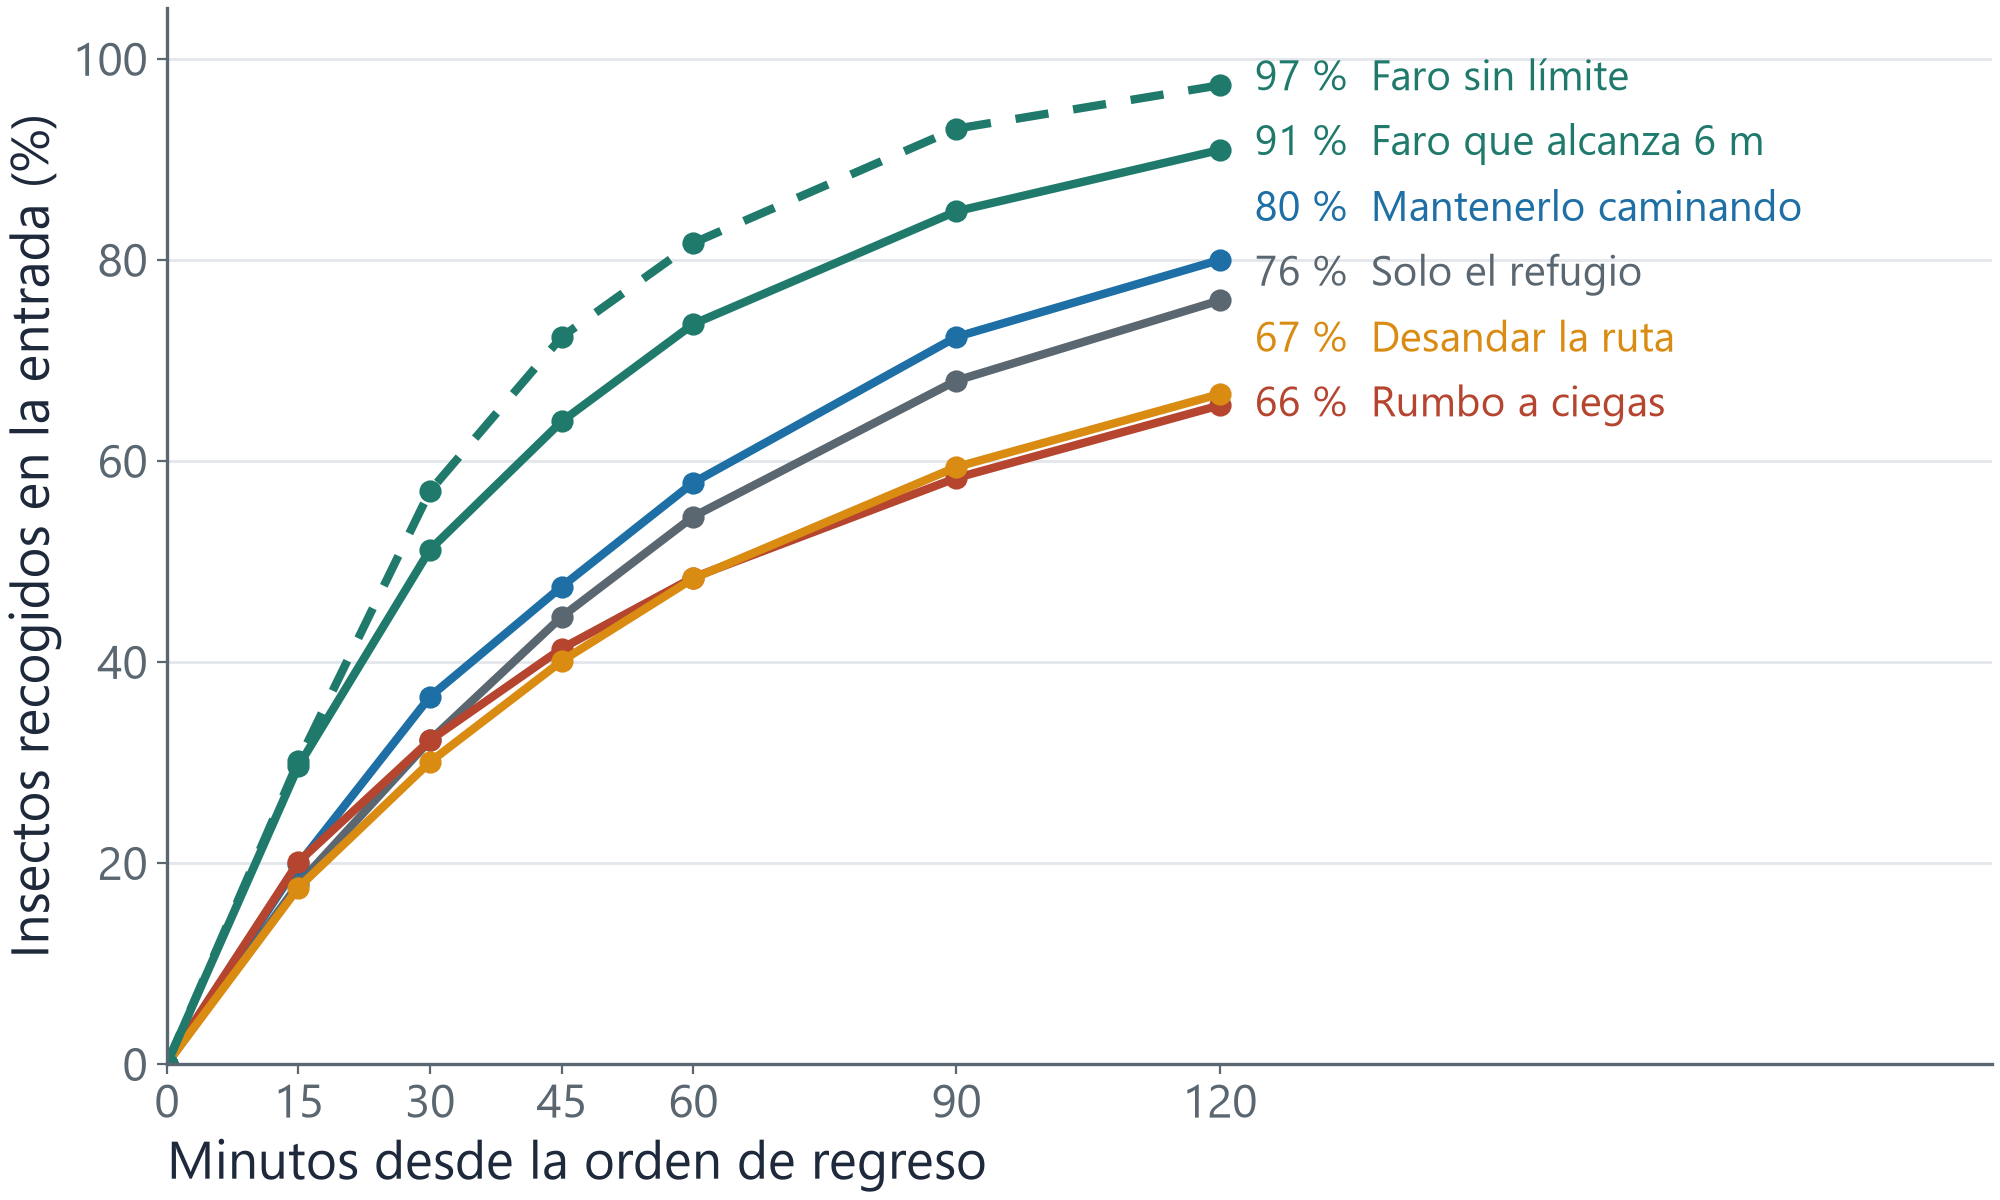
\includegraphics[width=0.70\textwidth]{figs/regreso.png}
\caption{Insectos recogidos en la entrada según la forma de hacerlos volver. La línea punteada es el techo del método.}
\label{fig:regreso}
\end{figure}

\textbf{Qué dice y qué no dice.} La guiada aumenta la detección en 45 a 60~min (de \pPasivaCuarentaCinco{} a
\pGuiadaCuarentaCinco~\% y de \pPasivaSesenta{} a \pGuiadaSesenta~\%) y lo hace con pocos estímulos, pero la mejora
depende del colapso. No dice cuánto tardaría un rescate real, porque los colapsos son planos y la marcha se midió en
arenas iluminadas, ni dice nada sobre falsas alarmas: en la simulación la persona es la única fuente de calor.


\subsection{Caso 4: el núcleo como circuito integrado}
\label{sec:layout}

Al final obtuvimos un GDS sin errores (figura~\ref{fig:layout} y tabla~\ref{tab:layout}). El chip mide $217.7\times228.4~\mu$m, es
decir \textbf{0.050~mm$^2$}, y consume \textbf{0.58~mA} a 1.8~V en espera. La frecuencia máxima la estimamos con el margen medido,
$f\approx1/(20~\text{ns}-\text{margen})$.

\begin{figure}[!htb]
\centering
\begin{subfigure}{0.42\textwidth}
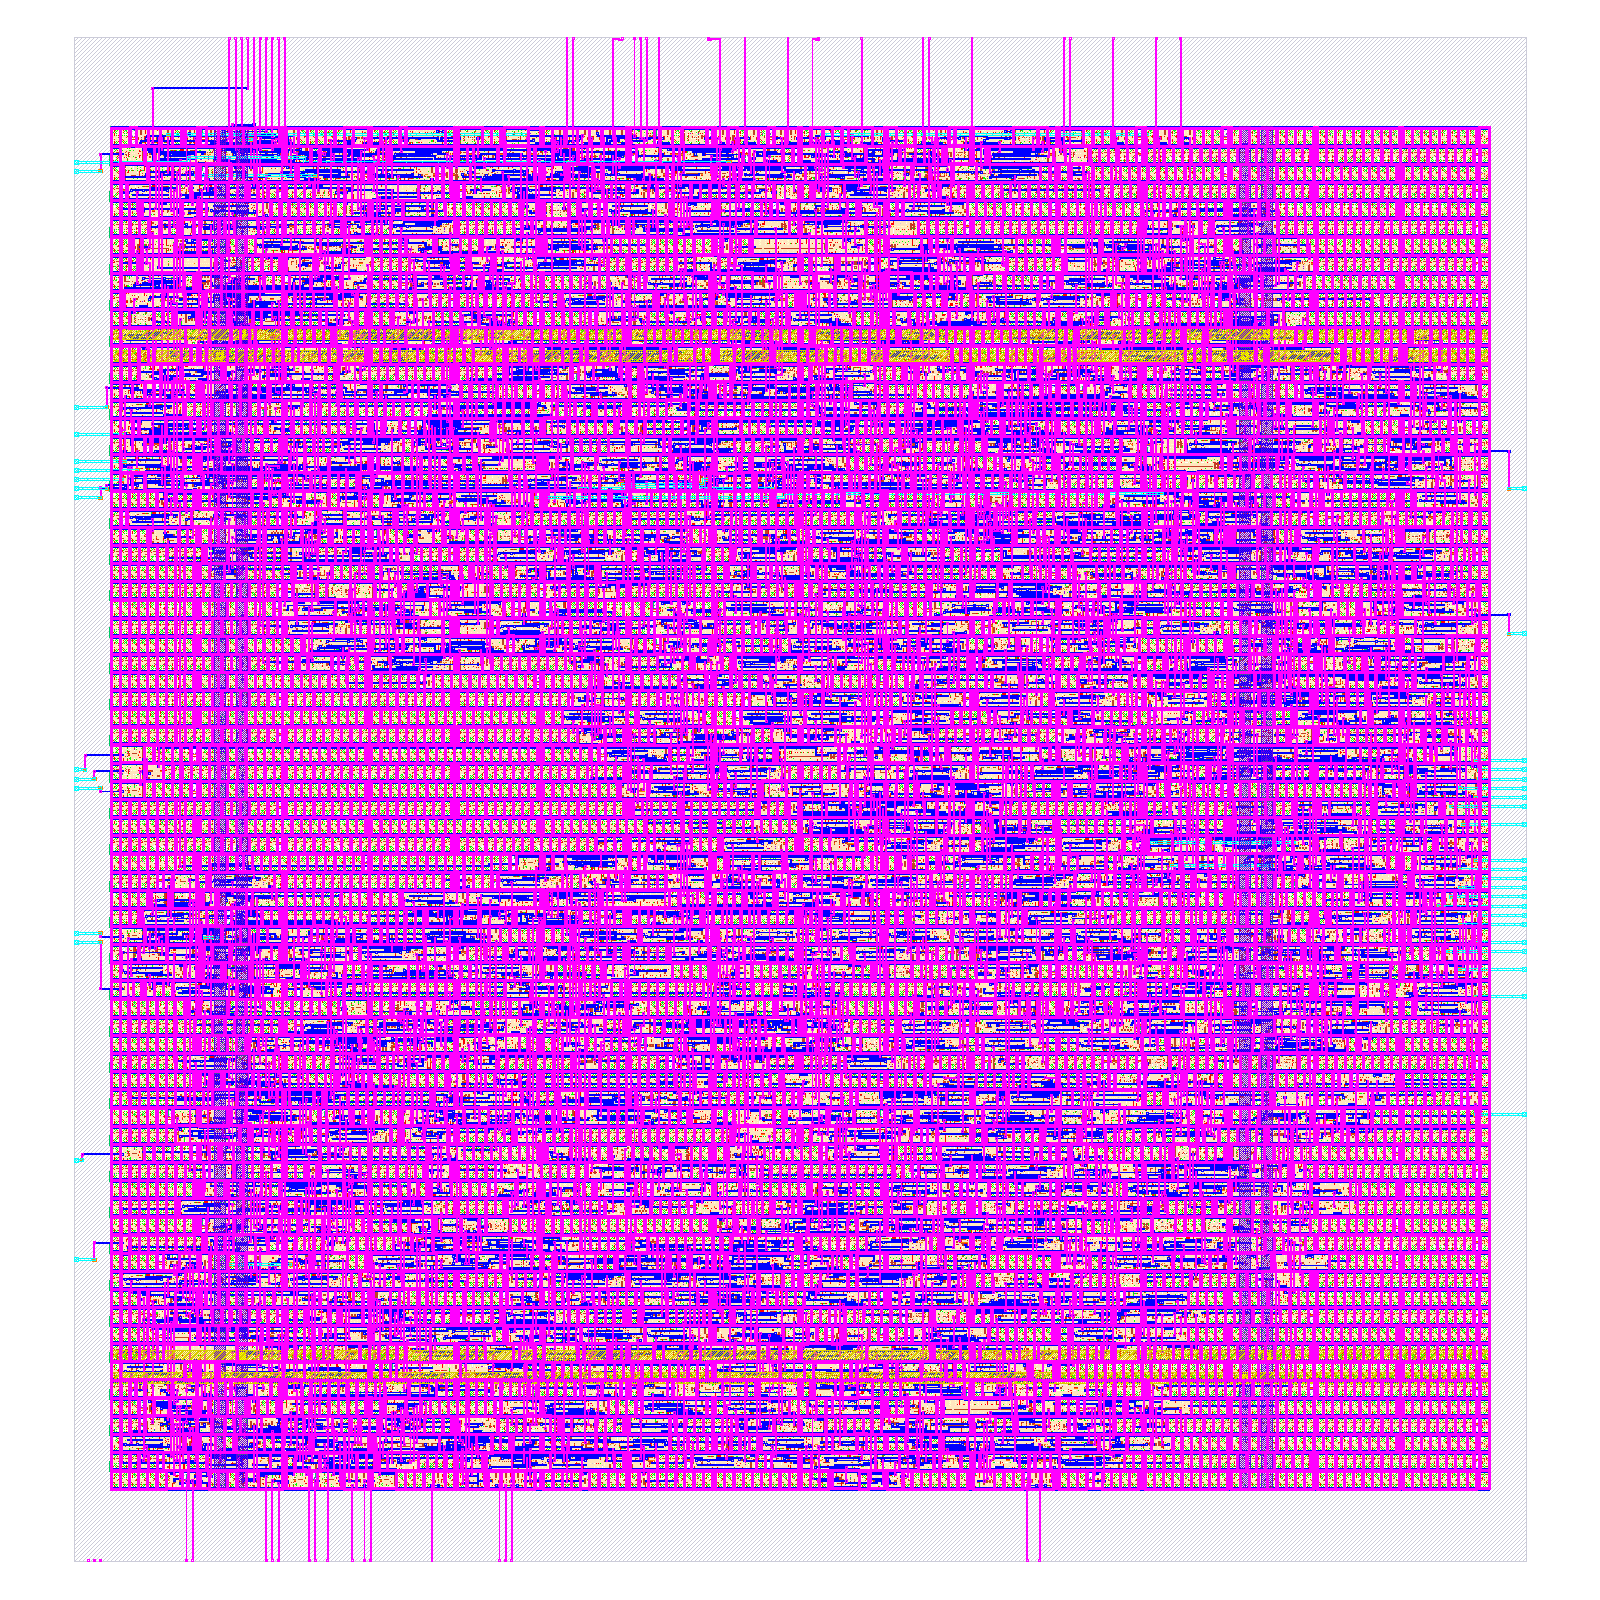
\includegraphics[width=\linewidth]{../layout/resultados/nucleo_biobot_klayout.png}
\caption{El dado: $217.7\times228.4~\mu$m.}
\end{subfigure}\hspace{0.04\textwidth}
\begin{subfigure}{0.42\textwidth}
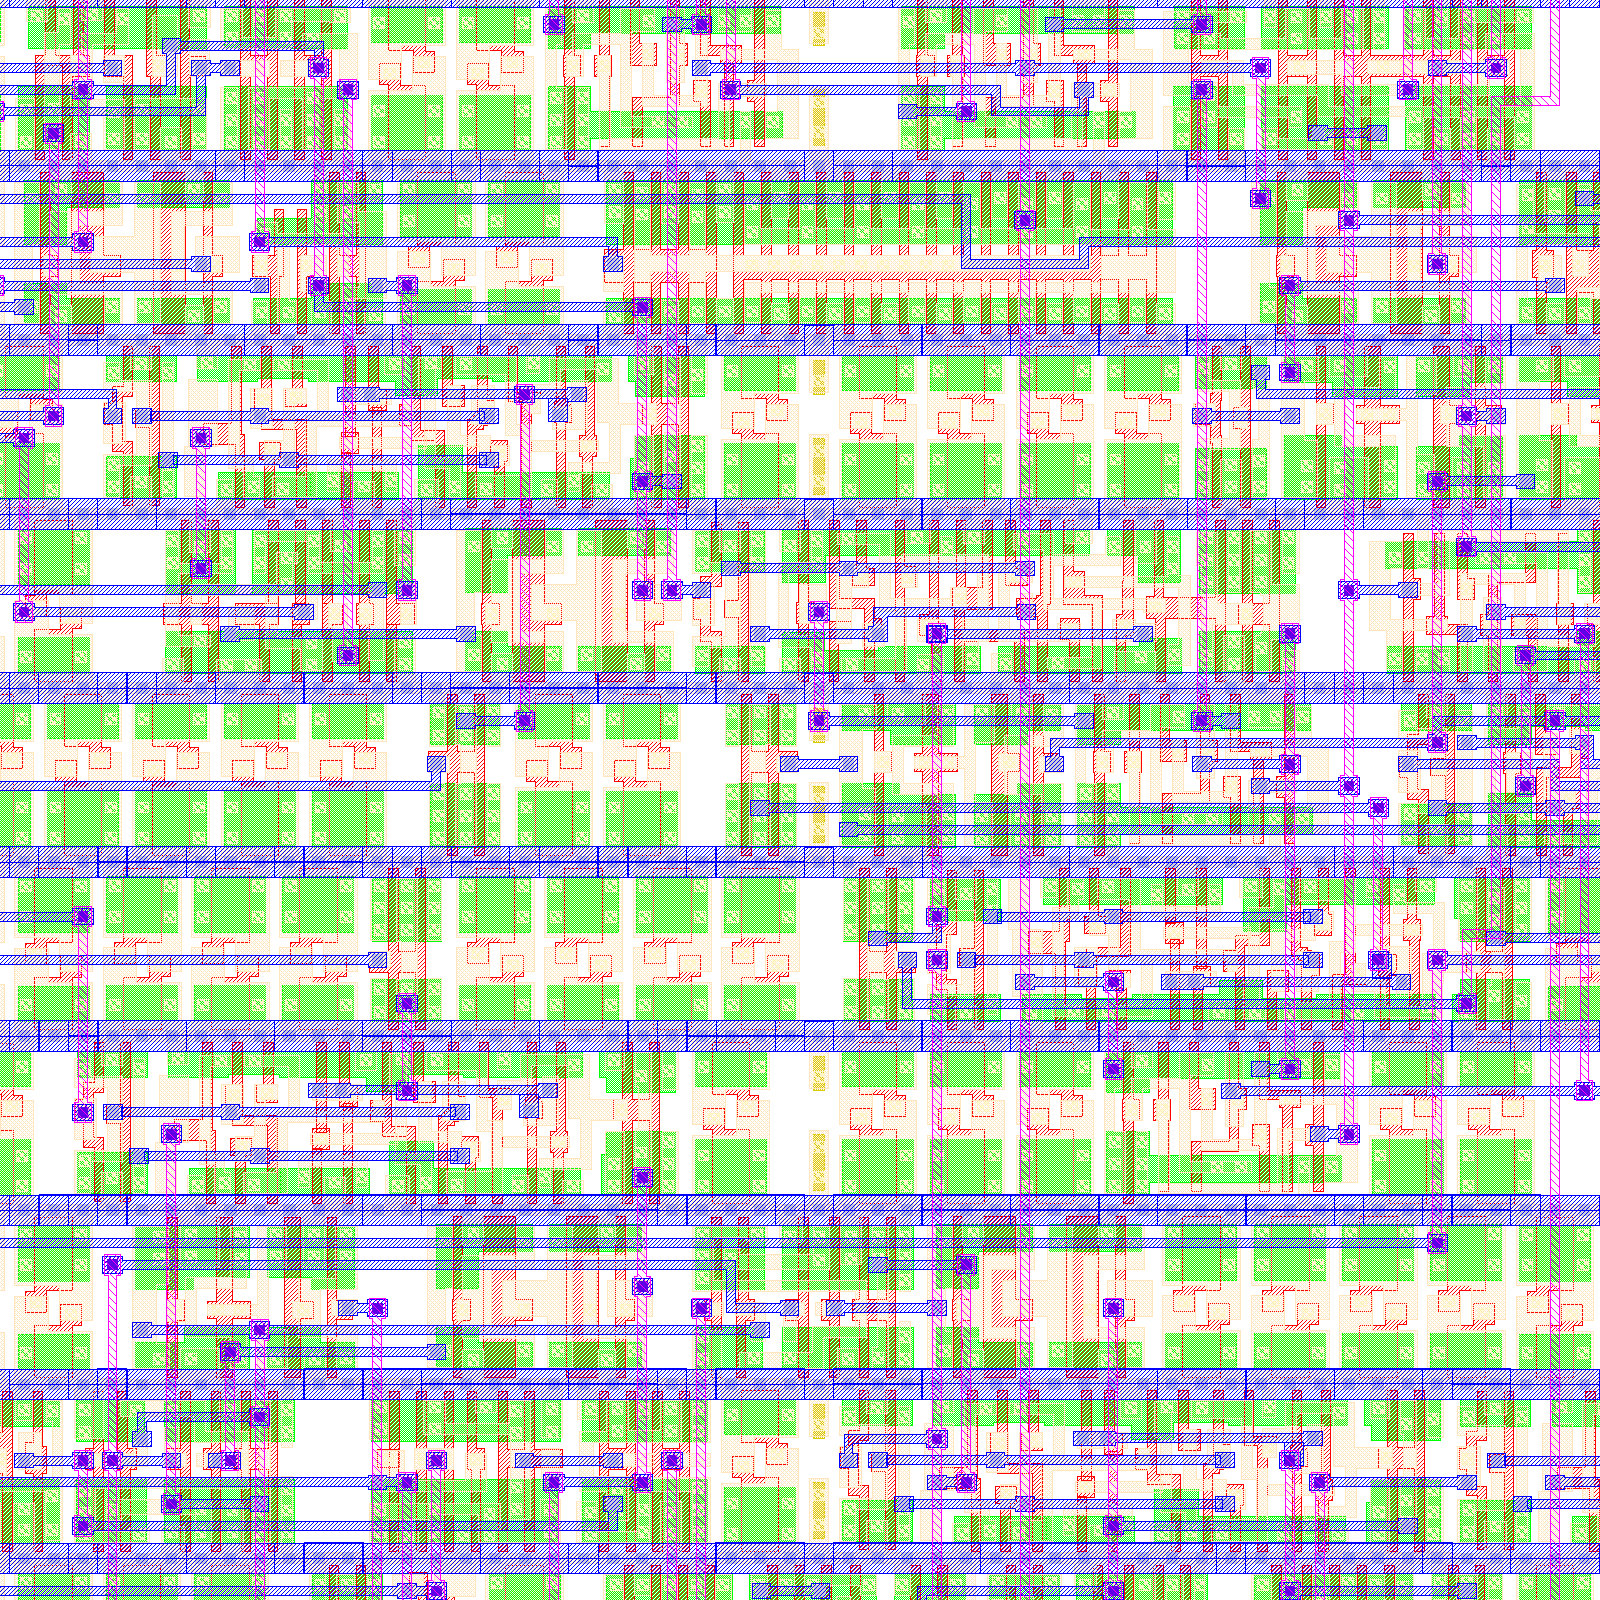
\includegraphics[width=\linewidth]{../layout/resultados/nucleo_biobot_detalle.png}
\caption{Acercamiento de $25\times25~\mu$m.}
\end{subfigure}

\medskip
\begin{subfigure}{0.42\textwidth}
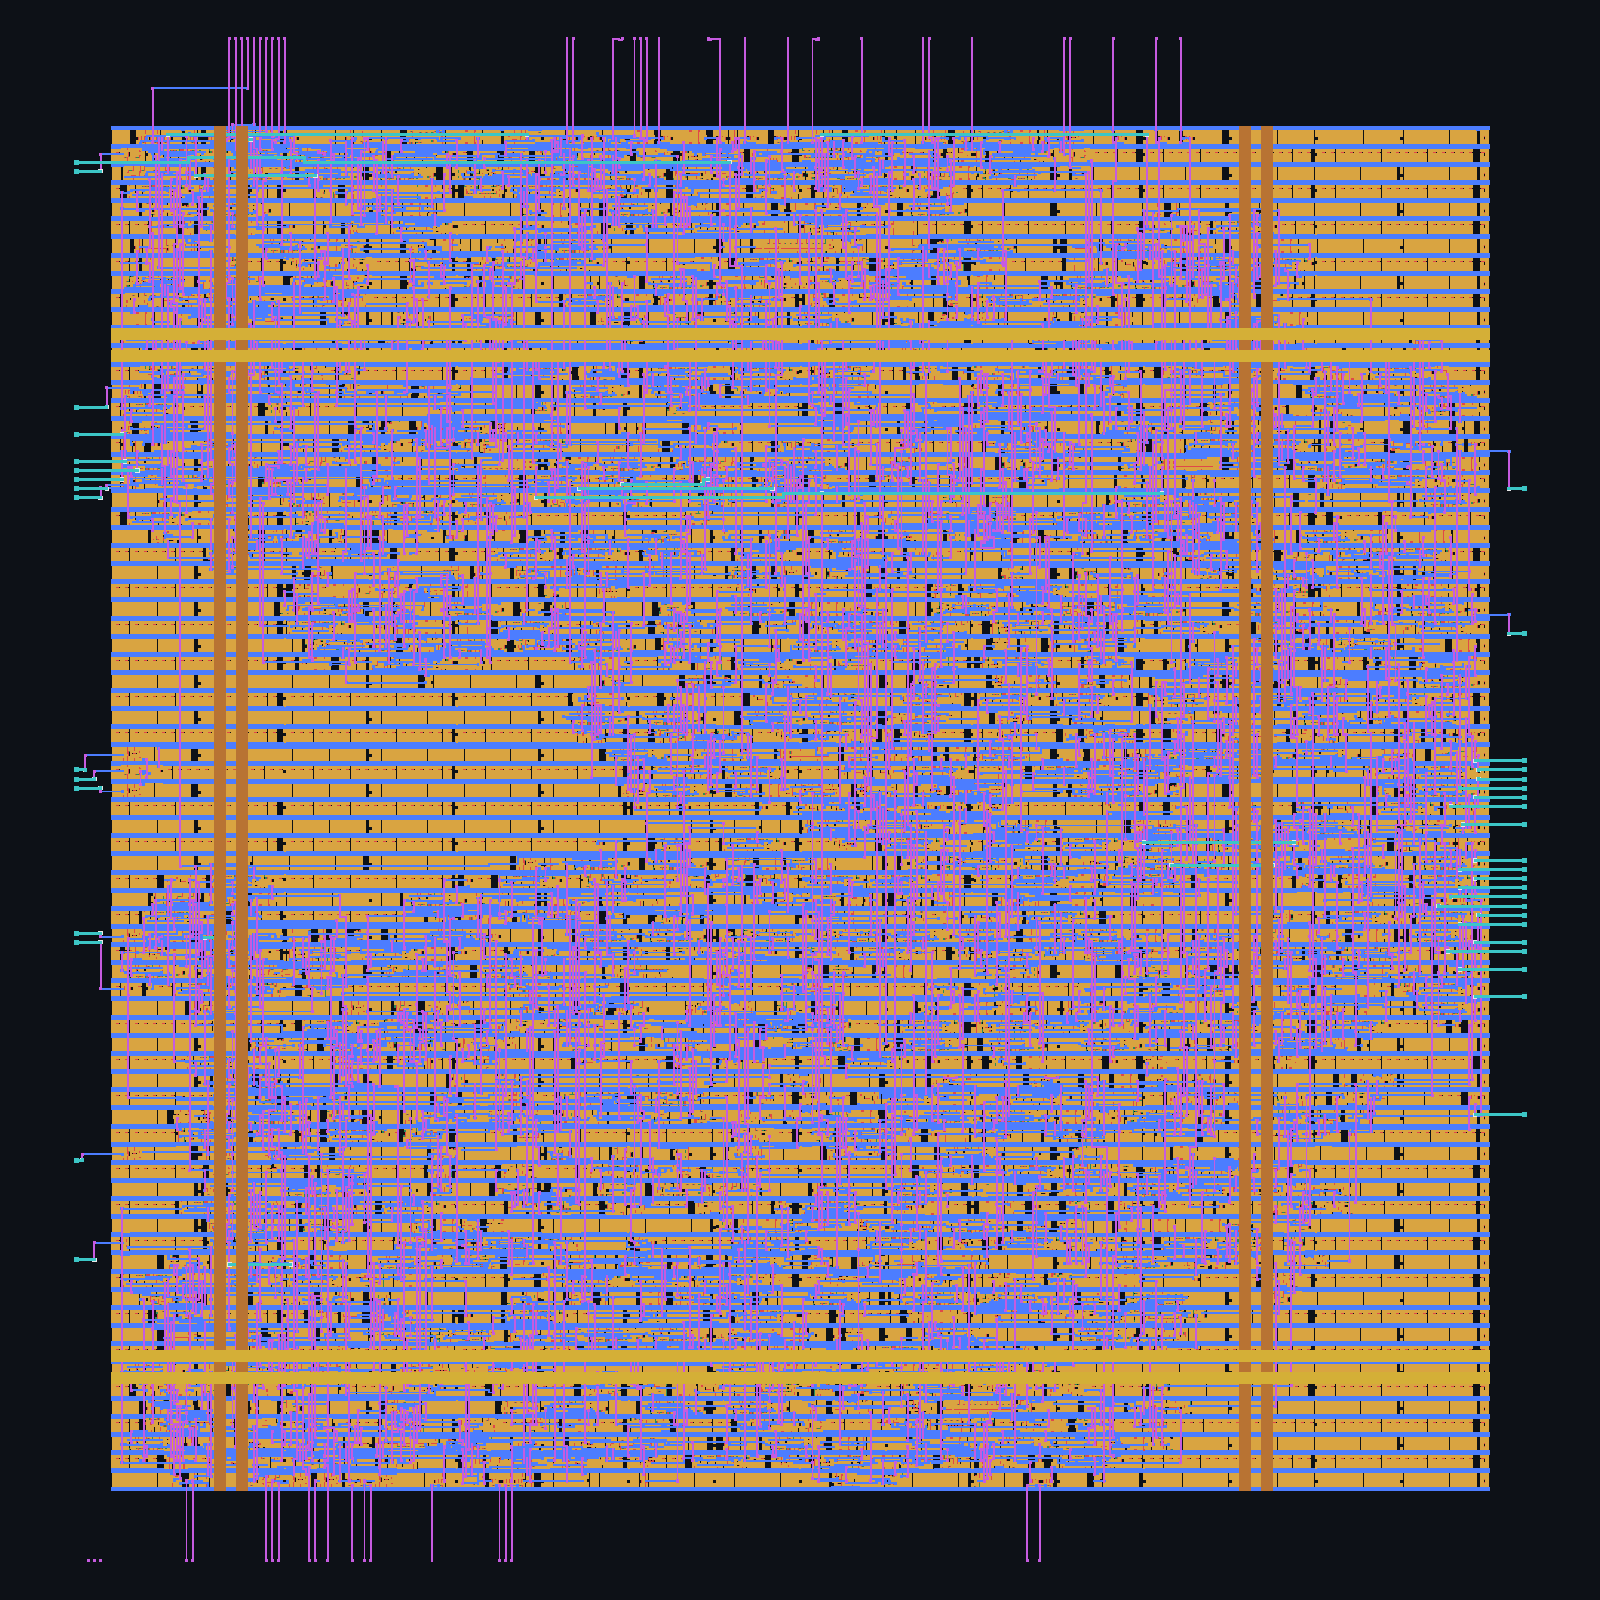
\includegraphics[width=\linewidth]{../layout/resultados/chip_color.png}
\caption{Los cinco metales y los pines.}
\end{subfigure}\hspace{0.04\textwidth}
\begin{subfigure}{0.42\textwidth}
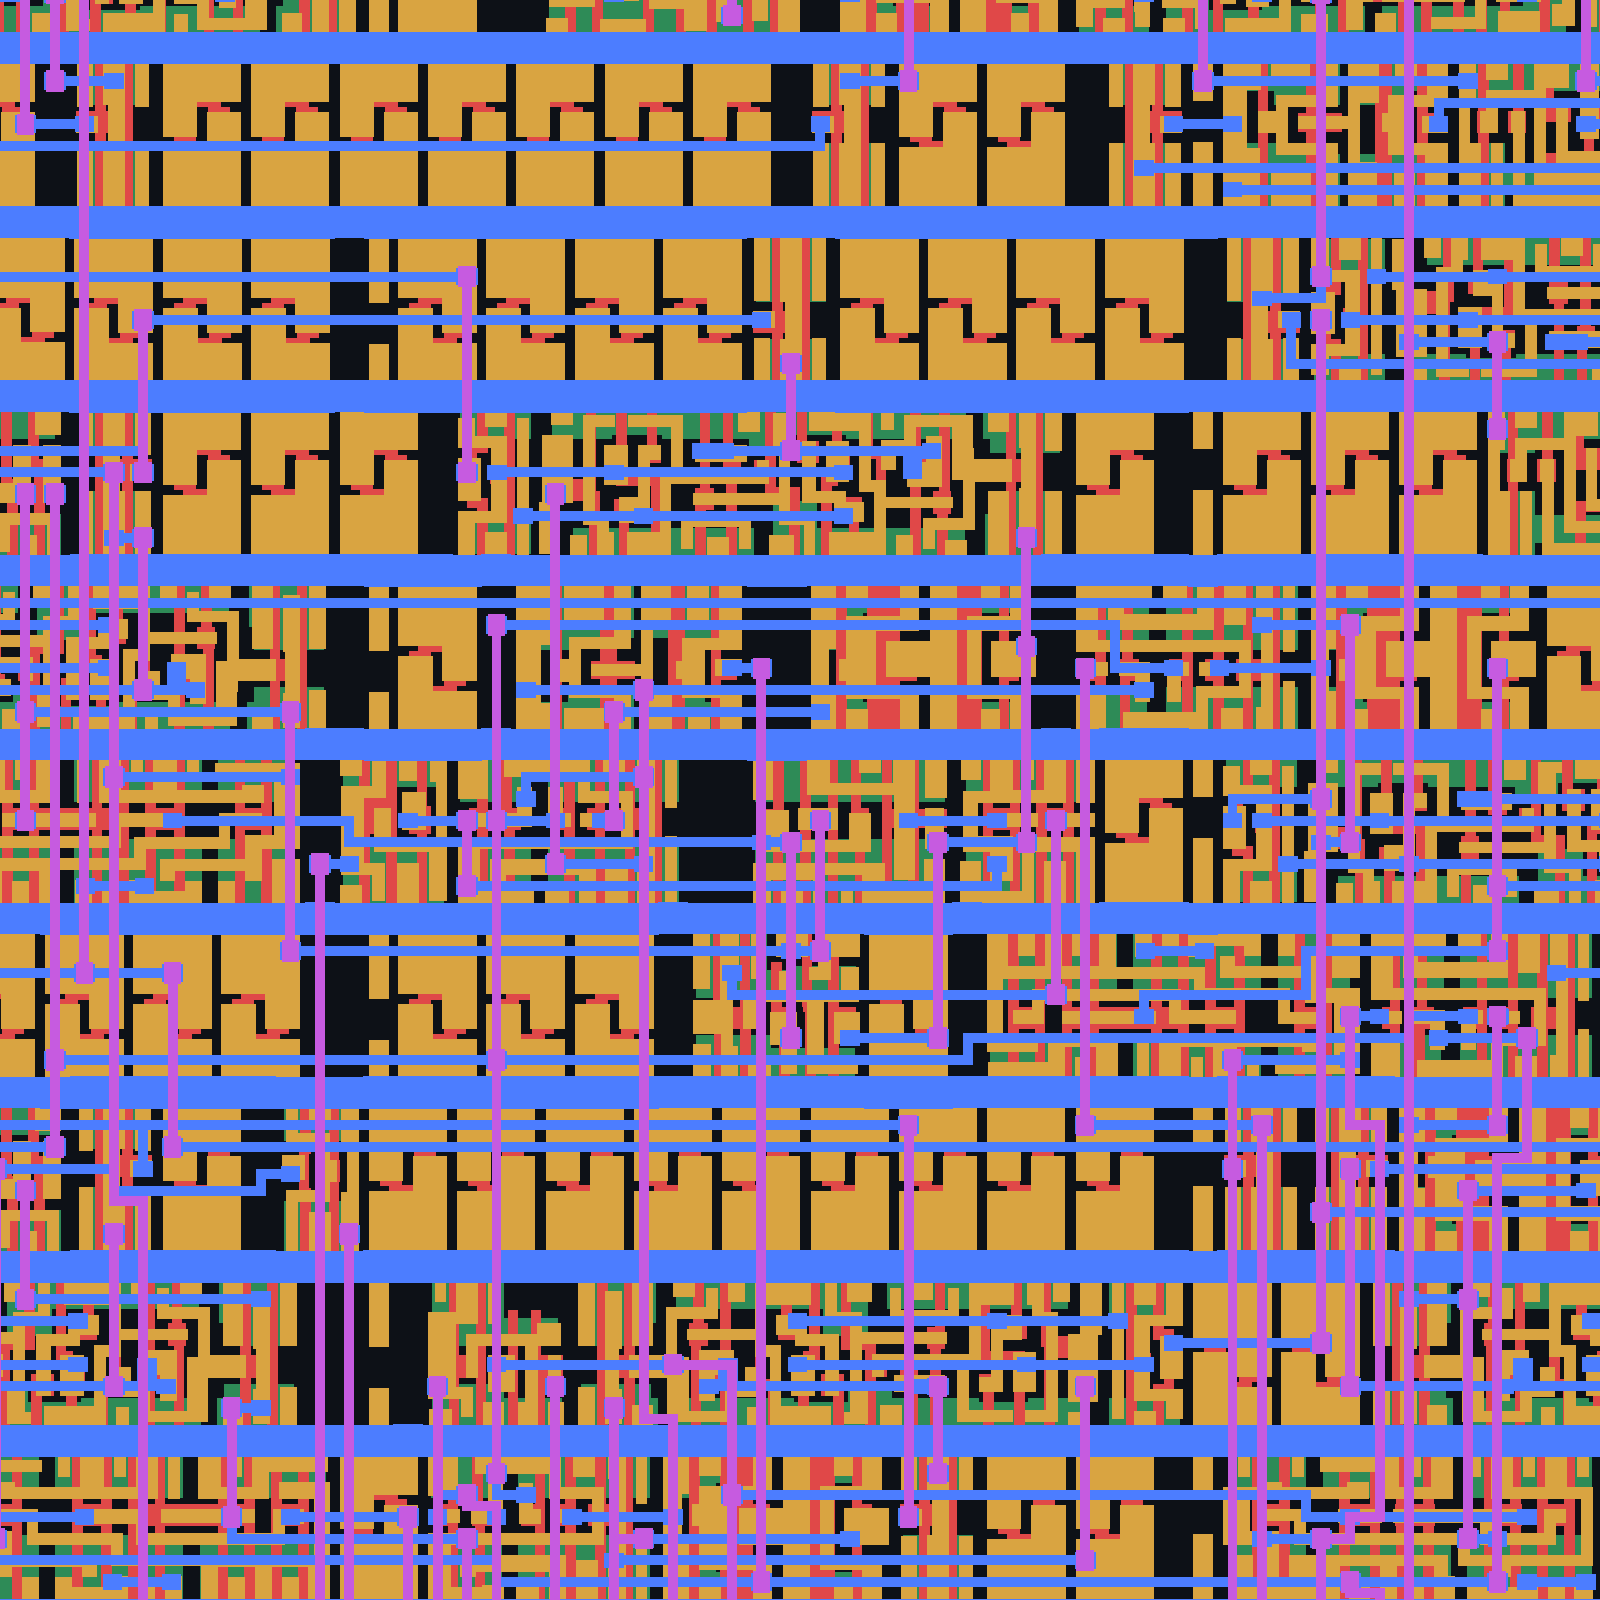
\includegraphics[width=\linewidth]{../layout/resultados/chip_color_acercamiento.png}
\caption{Acercamiento a las filas de celdas.}
\end{subfigure}
\caption{Layout del núcleo en SKY130: difusión (verde), polisilicio (rojo), interconexión local (crema), metal~1
(azul), metal~2 (magenta) y metal~3 (cian).}
\label{fig:layout}
\end{figure}

\begin{table}[!htb]
\centering\footnotesize
\caption{Resultados del layout (LibreLane 3.0.17, \sig{sky130\_fd\_sc\_hd}, reloj de 20~ns).}
\label{tab:layout}
\rowcolors{2}{SoftGray}{white}
\begin{tabularx}{0.92\textwidth}{@{}>{\raggedright\arraybackslash}X >{\raggedright\arraybackslash}p{7.0cm}@{}}
\toprule
\rowcolor{TableHead} \textbf{Medida} & \textbf{Valor} \\
\midrule
Área del dado; de las celdas colocadas & 0.050~mm$^2$; 0.023~mm$^2$ (ocupación de 53.7~\%) \\
Celdas estándar & 2\,671, de ellas 253 flip-flops \\
Búferes de reparación y de árbol de reloj & 485 y 67 \\
Margen de \emph{setup} y de \emph{hold}, peor esquina & +4.94~ns y +0.11~ns \\
Frecuencia máxima estimada & 72~MHz (lenta), 143~MHz (típica), 220~MHz (rápida) \\
Corriente a 1.8~V y 50~MHz, en espera & 0.577~mA (1.04~mW) \\
DRC (Magic y KLayout), LVS (Netgen) y antenas & 0 errores; los circuitos coinciden \\
\bottomrule
\end{tabularx}
\end{table}

\subsubsection{Área y consumo de corriente}
\label{sec:areacorriente}

\begin{figure}[!htb]
\centering
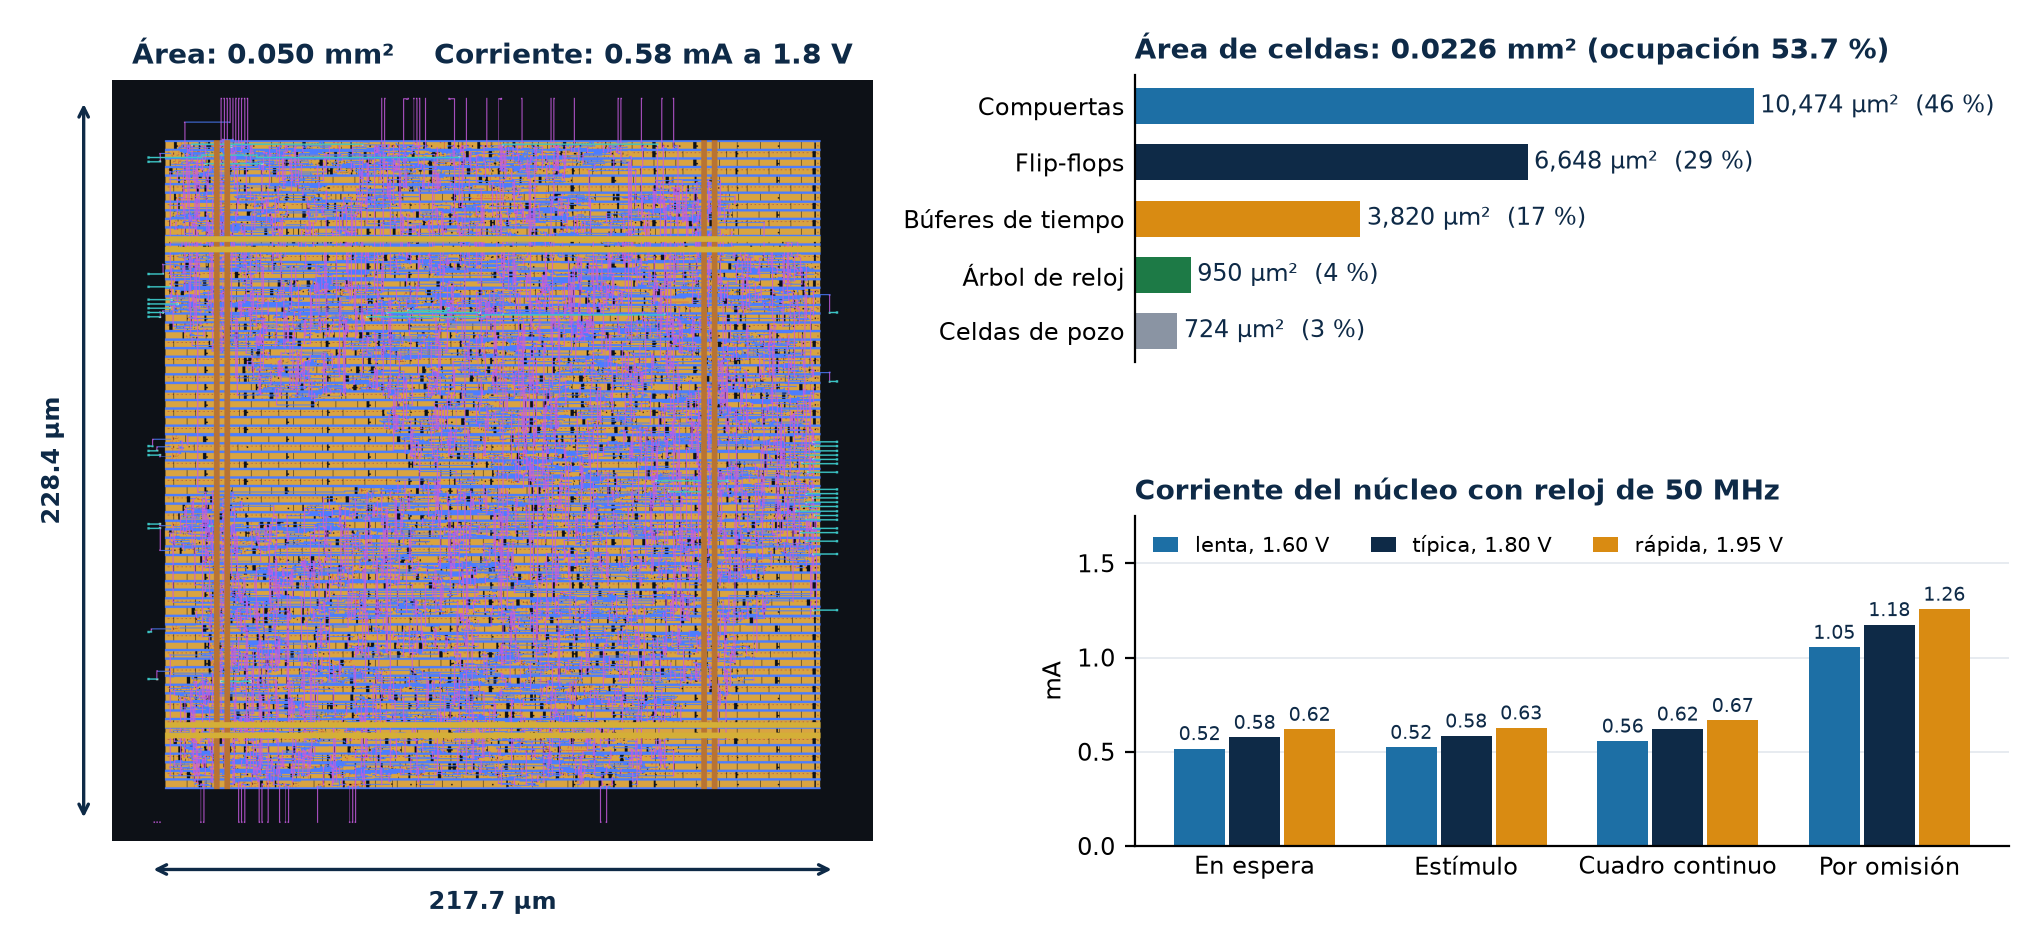
\includegraphics[width=\textwidth]{../layout/resultados/layout_area_corriente.png}
\caption{Área y corriente del layout: medidas del dado, reparto del área de celdas y corriente por esquina.}
\label{fig:areacorriente}
\end{figure}

El área la tomamos del layout terminado. Del dado, el núcleo interior ocupa 0.042~mm$^2$ y las celdas 0.0226~mm$^2$. De esas celdas,
el 46~\% son compuertas, el 29~\% flip-flops, el 17~\% búferes de tiempo, el 4~\% árbol de reloj y el 3~\% celdas de pozo
(figura~\ref{fig:areacorriente}). Para la corriente usamos OpenSTA sobre el netlist final, con los parásitos del ruteo, y la calculamos
de dos formas. Una usa la actividad de conmutación por omisión, que es la cota alta; la otra, la actividad real de una simulación del
netlist de compuertas, guardada en un VCD. Revisamos tres condiciones: en espera, con un tren de estímulo en curso y con cuadros
seguidos, un píxel por ciclo, que es el peor caso (tabla~\ref{tab:corriente}).

\begin{table}[!htb]
\centering\footnotesize
\caption{Potencia y corriente del núcleo a 50~MHz, $I=P/V_{DD}$.}
\label{tab:corriente}
\rowcolors{2}{SoftGray}{white}
\begin{tabularx}{\textwidth}{@{}>{\bfseries\raggedright\arraybackslash}X r r r r r r@{}}
\toprule
\rowcolor{TableHead} & \multicolumn{2}{c}{\textbf{Lenta, 1.60~V, 100~\textdegree C}} & \multicolumn{2}{c}{\textbf{Típica, 1.80~V, 25~\textdegree C}} & \multicolumn{2}{c}{\textbf{Rápida, 1.95~V, $-40$~\textdegree C}} \\
\rowcolor{TableHead} Condición & mW & mA & mW & mA & mW & mA \\
\midrule
En espera & 0.828 & 0.517 & 1.038 & 0.577 & 1.207 & 0.619 \\
Tren de estímulo & 0.838 & 0.524 & 1.051 & 0.584 & 1.222 & 0.627 \\
Cuadros seguidos & 0.891 & 0.557 & 1.117 & 0.621 & 1.299 & 0.666 \\
Actividad por omisión & 1.687 & 1.054 & 2.115 & 1.175 & 2.451 & 1.257 \\
Fuga & 0.0143 & 0.0090 & 0.00003 & 0.00001 & 0.00004 & 0.00002 \\
\bottomrule
\end{tabularx}
\end{table}

Casi toda la corriente se va en el reloj. En espera, la mitad la gasta su árbol y la otra mitad los flip-flops que lo
reciben, mientras que la lógica no llega a un microamperio. La potencia dinámica es proporcional a la frecuencia y el núcleo
solo procesa diez cuadros por segundo, así que con un reloj de 1~MHz gastaría unos 12~$\mu$A; el módulo ya recibe la
frecuencia como parámetro (\sig{CLK\_FREQ}). La caída en la red de alimentación es de 0.42~mV en el peor punto, el 0.02~\%
de 1.8~V.

\textbf{Frente a la FPGA y a la mochila.} Para tener con qué comparar usamos el analizador de Quartus. Sumando todas las alimentaciones
de la MAX~10, estima 63.5~mA para el prototipo del núcleo, 83.8~mA para la mochila de la red y 87.2~mA para el receptor. De eso, solo
4.4, 24.0 y 27.0~mA son dinámicos del núcleo lógico. Hay que tomarlo con cuidado, porque la propia herramienta marca la confianza como
baja al no tener actividad medida. Con el chip, ese consumo baja unas cien veces. Aun así, en la mochila completa, que gasta unos 30~mW (8.1~mA de una batería
de 3.7~V), el núcleo es apenas cerca del 3~\% de la potencia y lo demás se va sobre todo en el sensor y la radio.

